%!TEX TS-program = xelatex

\documentclass[oneside, openany]{memoir}


%\documentclass[a4paper,12pt]{article}

%%% Работа с русским языком
\usepackage[english,russian]{babel}   %% загружает пакет многоязыковой вёрстки
\usepackage{fontspec}      %% подготавливает загрузку шрифтов Open Type, True Type и др.
\defaultfontfeatures{Ligatures={TeX},Renderer=Basic}  %% свойства шрифтов по умолчанию
\setmainfont[Ligatures={TeX,Historic}]{Times New Roman} %% задаёт основной шрифт документа
\setsansfont{Comic Sans MS}                    %% задаёт шрифт без засечек
\setmonofont{Courier New}
\usepackage{indentfirst}
\frenchspacing

\renewcommand{\epsilon}{\ensuremath{\varepsilon}}
\renewcommand{\phi}{\ensuremath{\varphi}}
\renewcommand{\kappa}{\ensuremath{\varkappa}}
\renewcommand{\le}{\ensuremath{\leqslant}}
\renewcommand{\leq}{\ensuremath{\leqslant}}
\renewcommand{\ge}{\ensuremath{\geqslant}}
\renewcommand{\geq}{\ensuremath{\geqslant}}
\renewcommand{\emptyset}{\varnothing}

%%% Дополнительная работа с математикой
\usepackage{amsmath,amsfonts,amssymb,amsthm,mathtools} % AMS
\usepackage{icomma} % "Умная" запятая: $0,2$ --- число, $0, 2$ --- перечисление

%% Номера формул
%\mathtoolsset{showonlyrefs=true} % Показывать номера только у тех формул, на которые есть \eqref{} в тексте.
%\usepackage{leqno} % Нумерация формул слева

%% Свои команды
\DeclareMathOperator{\sgn}{\mathop{sgn}}

%% Перенос знаков в формулах (по Львовскому)
\newcommand*{\hm}[1]{#1\nobreak\discretionary{}
	{\hbox{$\mathsurround=0pt #1$}}{}}

%%% Работа с картинками
\usepackage{graphicx}  % Для вставки рисунков
\graphicspath{{images/}{images2/}}  % папки с картинками
\setlength\fboxsep{3pt} % Отступ рамки \fbox{} от рисунка
\setlength\fboxrule{1pt} % Толщина линий рамки \fbox{}
\usepackage{wrapfig} % Обтекание рисунков текстом

%%% Работа с таблицами
\usepackage{array,tabularx,tabulary,booktabs} % Дополнительная работа с таблицами
\usepackage{longtable}  % Длинные таблицы
\usepackage{multirow} % Слияние строк в таблице


%%% Программирование
\usepackage{etoolbox} % логические операторы


%%% Страница
\usepackage{extsizes} % Возможность сделать 14-й шрифт
\usepackage{geometry} % Простой способ задавать поля
\geometry{top=25mm}
\geometry{bottom=35mm}
\geometry{left=35mm}
\geometry{right=20mm}
%
%\usepackage{fancyhdr} % Колонтитулы
% 	\pagestyle{fancy}
%\renewcommand{\headrulewidth}{0pt}  % Толщина линейки, отчеркивающей верхний колонтитул
% 	\lfoot{Нижний левый}
% 	\rfoot{Нижний правый}
% 	\rhead{Верхний правый}
% 	\chead{Верхний в центре}
% 	\lhead{Верхний левый}
%	\cfoot{Нижний в центре} % По умолчанию здесь номер страницы

\usepackage{setspace} % Интерлиньяж
%\onehalfspacing % Интерлиньяж 1.5
%\doublespacing % Интерлиньяж 2
%\singlespacing % Интерлиньяж 1

\usepackage{lastpage} % Узнать, сколько всего страниц в документе.

\usepackage{soul} % Модификаторы начертания

\usepackage{hyperref}
\usepackage[usenames,dvipsnames,svgnames,table,rgb]{xcolor}
\hypersetup{				% Гиперссылки
	unicode=true,           % русские буквы в раздела PDF
	pdftitle={Заголовок},   % Заголовок
	pdfauthor={Автор},      % Автор
	pdfsubject={Тема},      % Тема
	pdfcreator={Создатель}, % Создатель
	pdfproducer={Производитель}, % Производитель
	pdfkeywords={keyword1} {key2} {key3}, % Ключевые слова
	colorlinks=true,       	% false: ссылки в рамках; true: цветные ссылки
	linkcolor=red,          % внутренние ссылки
	citecolor=black,        % на библиографию
	filecolor=magenta,      % на файлы
	urlcolor=cyan           % на URL
}

\usepackage{csquotes} % Еще инструменты для ссылок

%\usepackage[style=authoryear,maxcitenames=2,backend=biber,sorting=nty]{biblatex}

\usepackage{multicol} % Несколько колонок

\usepackage{tikz} % Работа с графикой
\usepackage{pgfplots}
\usepackage{pgfplotstable}


\usepackage{markdown}

\author{версия 0.2}
\title{Простые решения уравнения фильтрации}
\date{\today}

%%% Реализация библиографии пакетами biblatex и biblatex-gost с использованием движка biber %%%

\usepackage{csquotes} % biblatex рекомендует его подключать. Пакет для оформления сложных блоков цитирования.

\usepackage[%
	backend=biber,% движок
	bibencoding=utf8,% кодировка bib файла
	sorting=none,% настройка сортировки списка литературы
	style=gost-numeric,% стиль цитирования и библиографии (по ГОСТ)
	language=autobib,% получение языка из babel/polyglossia, default: autobib % если ставить autocite или auto, то цитаты в тексте с указанием страницы, получат указание страницы на языке оригинала
	autolang=other,% многоязычная библиография
	clearlang=true,% внутренний сброс поля language, если он совпадает с языком из babel/polyglossia
	defernumbers=true,% нумерация проставляется после двух компиляций, зато позволяет выцеплять библиографию по ключевым словам и нумеровать не из большего списка
	sortcites=true,% сортировать номера затекстовых ссылок при цитировании (если в квадратных скобках несколько ссылок, то отображаться будут отсортированно, а не абы как)
	doi=true,% Показывать или нет ссылки на DOI
	isbn=false,% Показывать или нет ISBN, ISSN, ISRN
	movenames = false,
	maxnames = 10,
	]{biblatex}[2016/09/17]





%%% Подключение файлов bib %%%
\addbibresource[label=papers]{biblio/biblio_papers.bib}
\addbibresource[label=books]{biblio/biblio_books.bib}


%http://tex.stackexchange.com/a/141831/79756
%There is a way to automatically map the language field to the langid field. The following lines in the preamble should be enough to do that.
%This command will copy the language field into the langid field and will then delete the contents of the language field. The language field will only be deleted if it was successfully copied into the langid field.
\DeclareSourcemap{ %модификация bib файла перед тем, как им займётся biblatex
	\maps{
		\map{% перекидываем значения полей language в поля langid, которыми пользуется biblatex
			\step[fieldsource=language, fieldset=langid, origfieldval, final]
			\step[fieldset=language, null]
		}
		\map{% перекидываем значения полей numpages в поля pagetotal, которыми пользуется biblatex
			\step[fieldsource=numpages, fieldset=pagetotal, origfieldval, final]
			\step[fieldset=numpages, null]
		}
		\map{% перекидываем значения полей pagestotal в поля pagetotal, которыми пользуется biblatex
			\step[fieldsource=pagestotal, fieldset=pagetotal, origfieldval, final]
			\step[fieldset=pagestotal, null]
		}
		\map[overwrite]{% перекидываем значения полей shortjournal, если они есть, в поля journal, которыми пользуется biblatex
			\step[fieldsource=shortjournal, final]
			\step[fieldset=journal, origfieldval]
			\step[fieldset=shortjournal, null]
		}
		\map[overwrite]{% перекидываем значения полей shortbooktitle, если они есть, в поля booktitle, которыми пользуется biblatex
			\step[fieldsource=shortbooktitle, final]
			\step[fieldset=booktitle, origfieldval]
			\step[fieldset=shortbooktitle, null]
		}
		\map{% если в поле medium написано "Электронный ресурс", то устанавливаем поле media, которым пользуется biblatex, в значение eresource.
			\step[fieldsource=medium,
			match=\regexp{Электронный\s+ресурс},
			final]
			\step[fieldset=media, fieldvalue=eresource]
			\step[fieldset=medium, null]
		}
	%	\map{% использование media=text по умолчанию
	%		\step[fieldset=media, fieldvalue=text]
	%	}
		\map[overwrite]{% стираем значения всех полей issn
			\step[fieldset=issn, null]
		}
		\map[overwrite]{% стираем значения всех полей abstract, поскольку ими не пользуемся, а там бывают "неприятные" латеху символы
			\step[fieldsource=abstract]
			\step[fieldset=abstract,null]
		}
		\map[overwrite]{ % переделка формата записи даты
			\step[fieldsource=urldate,
			match=\regexp{([0-9]{2})\.([0-9]{2})\.([0-9]{4})},
			replace={$3-$2-$1$4}, % $4 вставлен исключительно ради нормальной работы программ подсветки синтаксиса, которые некорректно обрабатывают $ в таких конструкциях
			final]
		}
		\map[overwrite]{ % стираем ключевые слова
			\step[fieldsource=keywords]
			\step[fieldset=keywords,null]
		}
		% реализация foreach различается для biblatex v3.12 и v3.13.
		% Для версии v3.13 эта конструкция заменяет последующие 5 структур map
		% \map[overwrite,foreach={authorvak,authorscopus,authorwos,authorconf,authorother}]{ % записываем информацию о типе публикации в ключевые слова
		%     \step[fieldsource=$MAPLOOP,final=true]
		%     \step[fieldset=keywords,fieldvalue={,biblio$MAPLOOP},append=true]
		% }
		\map[overwrite]{ % записываем информацию о типе публикации в ключевые слова
			\step[fieldsource=authorvak,final=true]
			\step[fieldset=keywords,fieldvalue={,biblioauthorvak},append=true]
		}
		\map[overwrite]{ % записываем информацию о типе публикации в ключевые слова
			\step[fieldsource=authorscopus,final=true]
			\step[fieldset=keywords,fieldvalue={,biblioauthorscopus},append=true]
		}
		\map[overwrite]{ % записываем информацию о типе публикации в ключевые слова
			\step[fieldsource=authorwos,final=true]
			\step[fieldset=keywords,fieldvalue={,biblioauthorwos},append=true]
		}
		\map[overwrite]{ % записываем информацию о типе публикации в ключевые слова
			\step[fieldsource=authorconf,final=true]
			\step[fieldset=keywords,fieldvalue={,biblioauthorconf},append=true]
		}
		\map[overwrite]{ % записываем информацию о типе публикации в ключевые слова
			\step[fieldsource=authorother,final=true]
			\step[fieldset=keywords,fieldvalue={,biblioauthorother},append=true]
		}
		\map[overwrite]{ % добавляем ключевые слова, чтобы различать источники
			\perdatasource{biblio/external.bib}
			\step[fieldset=keywords, fieldvalue={,biblioexternal},append=true]
		}
		\map[overwrite]{ % добавляем ключевые слова, чтобы различать источники
			\perdatasource{biblio/author.bib}
			\step[fieldset=keywords, fieldvalue={,biblioauthor},append=true]
		}
		\map[overwrite]{ % добавляем ключевые слова, чтобы различать источники
			\step[fieldset=keywords, fieldvalue={,bibliofull},append=true]
		}
		%        \map[overwrite]{% стираем значения всех полей series
		%            \step[fieldset=series, null]
		%        }
		\map[overwrite]{% перекидываем значения полей howpublished в поля organization для типа online
			\step[typesource=online, typetarget=online, final]
			\step[fieldsource=howpublished, fieldset=organization, origfieldval]
			\step[fieldset=howpublished, null]
		}
		% Так отключаем [Электронный ресурс]
		%        \map[overwrite]{% стираем значения всех полей media=eresource
		%            \step[fieldsource=media,
		%            match={eresource},
		%            final]
		%            \step[fieldset=media, null]
		%        }
	}
}



\defbibfilter{vakscopuswos}{%
	keyword=biblioauthorvak or keyword=biblioauthorscopus or keyword=biblioauthorwos
}

\defbibfilter{scopuswos}{%
	keyword=biblioauthorscopus or keyword=biblioauthorwos
}

%%% Тире как разделитель в библиографии традиционной руской длины:
\renewcommand*{\newblockpunct}{\addperiod\addnbspace\cyrdash\space\bibsentence}

%%% В списке литературы обозначение одной буквой диапазона страниц англоязычного источника %%%
\DefineBibliographyStrings{english}{%
	pages = {p\adddot} %заглавность буквы затем по месту определяется работой самого biblatex
}

%%% Исправление длины тире в диапазонах %%%
% \cyrdash --- тире «русской» длины, \textendash --- en-dash
\DefineBibliographyExtras{russian}{%
	\protected\def\bibrangedash{%
		\cyrdash\penalty\value{abbrvpenalty}}% almost unbreakable dash
	\protected\def\bibdaterangesep{\bibrangedash}%тире для дат
}
\DefineBibliographyExtras{english}{%
	\protected\def\bibrangedash{%
		\cyrdash\penalty\value{abbrvpenalty}}% almost unbreakable dash
	\protected\def\bibdaterangesep{\bibrangedash}%тире для дат
}









\begin{document} % конец преамбулы, начало документа
	
	\maketitle
	
	
	
	\chapter{Стационарные решения уравнения фильтрации}
	
	Широкое распространение на практике получили стационарные решения уравнения фильтрации. Приведем некоторые из них.

\section{Решение для постоянного давления на круговой границе}

Рассматривается самая простая модель работы добывающей скважины - радиальная стационарная фильтрация в однородном изотропном пласте круговой формы. Скважина находится в центре пласта (рис. \ref{ris:radial_inflow_steady_state_1}). На границе пласта поддерживается постоянное давление. Фактически это означает, что через границу пласта идет поток жидкости, уравновешивающий дебит скважины. 

Решение можно получить как решения уравнения фильтрации, учитывая стационарность потока

\begin{equation} \label{eq:diff_eq_1} 
	\frac{\partial ^2 p }{\partial r^2} + \frac{1}{r} \frac{\partial p}{\partial r} = 0
\end{equation}

  

\begin{figure}[h!]
	\begin{center}
		

\tikzset{every picture/.style={line width=0.75pt}} %set default line width to 0.75pt        

\begin{tikzpicture}[x=0.75pt,y=0.75pt,yscale=-1,xscale=1]
%uncomment if require: \path (0,493); %set diagram left start at 0, and has height of 493

%Shape: Rectangle [id:dp2210940442519349] 
\draw  [color={rgb, 255:red, 74; green, 144; blue, 226 }  ,draw opacity=1 ] (297.5,90) -- (432.5,90) -- (432.5,151) -- (297.5,151) -- cycle ;
%Shape: Circle [id:dp04970297189708517] 
\draw  [color={rgb, 255:red, 74; green, 144; blue, 226 }  ,draw opacity=1 ][fill={rgb, 255:red, 255; green, 255; blue, 255 }  ,fill opacity=1 ] (297.5,345) .. controls (297.5,307.72) and (327.72,277.5) .. (365,277.5) .. controls (402.28,277.5) and (432.5,307.72) .. (432.5,345) .. controls (432.5,382.28) and (402.28,412.5) .. (365,412.5) .. controls (327.72,412.5) and (297.5,382.28) .. (297.5,345) -- cycle ;
%Shape: Circle [id:dp10293196217835776] 
\draw   (247.5,345) .. controls (247.5,280.11) and (300.11,227.5) .. (365,227.5) .. controls (429.89,227.5) and (482.5,280.11) .. (482.5,345) .. controls (482.5,409.89) and (429.89,462.5) .. (365,462.5) .. controls (300.11,462.5) and (247.5,409.89) .. (247.5,345) -- cycle ;
%Shape: Rectangle [id:dp45852916067627625] 
\draw   (247.5,90) -- (482.5,90) -- (482.5,151) -- (247.5,151) -- cycle ;
%Shape: Rectangle [id:dp1911911198156271] 
\draw  [color={rgb, 255:red, 255; green, 255; blue, 255 }  ,draw opacity=1 ][fill={rgb, 255:red, 255; green, 255; blue, 255 }  ,fill opacity=1 ] (350,79.5) -- (380,79.5) -- (380,100.5) -- (350,100.5) -- cycle ;
%Shape: Circle [id:dp188351868386184] 
\draw   (350,345) .. controls (350,336.72) and (356.72,330) .. (365,330) .. controls (373.28,330) and (380,336.72) .. (380,345) .. controls (380,353.28) and (373.28,360) .. (365,360) .. controls (356.72,360) and (350,353.28) .. (350,345) -- cycle ;
%Straight Lines [id:da05843072951767869] 
\draw  [dash pattern={on 0.84pt off 2.51pt}]  (247.5,151) -- (247.5,345) ;
%Straight Lines [id:da5104578805624558] 
\draw  [dash pattern={on 0.84pt off 2.51pt}]  (482.5,151) -- (482.5,345) ;
%Straight Lines [id:da6468348992509316] 
\draw    (350,70) -- (350,90) ;
%Straight Lines [id:da34061741935451995] 
\draw    (380,70) -- (380,90) ;
%Straight Lines [id:da792017081317731] 
\draw  [dash pattern={on 0.84pt off 2.51pt}]  (365,90) -- (365,345) ;
%Straight Lines [id:da9746844382077546] 
\draw    (365,345) -- (430.75,436.32) ;
\draw [shift={(432.5,438.75)}, rotate = 234.25] [fill={rgb, 255:red, 0; green, 0; blue, 0 }  ][line width=0.08]  [draw opacity=0] (7.14,-3.43) -- (0,0) -- (7.14,3.43) -- cycle    ;
%Straight Lines [id:da25168233148692076] 
\draw    (365,345) -- (423.22,368.86) ;
\draw [shift={(426,370)}, rotate = 202.29] [fill={rgb, 255:red, 0; green, 0; blue, 0 }  ][line width=0.08]  [draw opacity=0] (7.14,-3.43) -- (0,0) -- (7.14,3.43) -- cycle    ;
%Straight Lines [id:da9459663069624791] 
\draw    (368,170) -- (429.5,170) ;
\draw [shift={(432.5,170)}, rotate = 180] [fill={rgb, 255:red, 0; green, 0; blue, 0 }  ][line width=0.08]  [draw opacity=0] (7.14,-3.43) -- (0,0) -- (7.14,3.43) -- cycle    ;
\draw [shift={(365,170)}, rotate = 0] [fill={rgb, 255:red, 0; green, 0; blue, 0 }  ][line width=0.08]  [draw opacity=0] (7.14,-3.43) -- (0,0) -- (7.14,3.43) -- cycle    ;
%Straight Lines [id:da9708245914645104] 
\draw    (368,192) -- (479.5,192) ;
\draw [shift={(482.5,192)}, rotate = 180] [fill={rgb, 255:red, 0; green, 0; blue, 0 }  ][line width=0.08]  [draw opacity=0] (7.14,-3.43) -- (0,0) -- (7.14,3.43) -- cycle    ;
\draw [shift={(365,192)}, rotate = 0] [fill={rgb, 255:red, 0; green, 0; blue, 0 }  ][line width=0.08]  [draw opacity=0] (7.14,-3.43) -- (0,0) -- (7.14,3.43) -- cycle    ;
%Straight Lines [id:da320252059166237] 
\draw    (365,70) -- (365,44.25) ;
\draw [shift={(365,41.25)}, rotate = 450] [fill={rgb, 255:red, 0; green, 0; blue, 0 }  ][line width=0.08]  [draw opacity=0] (7.14,-3.43) -- (0,0) -- (7.14,3.43) -- cycle    ;
%Straight Lines [id:da2674421622778862] 
\draw    (237,120.5) -- (255.2,120.5) ;
\draw [shift={(258.2,120.5)}, rotate = 180] [fill={rgb, 255:red, 0; green, 0; blue, 0 }  ][line width=0.08]  [draw opacity=0] (7.14,-3.43) -- (0,0) -- (7.14,3.43) -- cycle    ;
%Straight Lines [id:da8177707390860813] 
\draw    (286.9,120.5) -- (305.1,120.5) ;
\draw [shift={(308.1,120.5)}, rotate = 180] [fill={rgb, 255:red, 0; green, 0; blue, 0 }  ][line width=0.08]  [draw opacity=0] (7.14,-3.43) -- (0,0) -- (7.14,3.43) -- cycle    ;
%Straight Lines [id:da17218179619021767] 
\draw    (445.95,120.5) -- (422.1,120.5) ;
\draw [shift={(419.1,120.5)}, rotate = 360] [fill={rgb, 255:red, 0; green, 0; blue, 0 }  ][line width=0.08]  [draw opacity=0] (7.14,-3.43) -- (0,0) -- (7.14,3.43) -- cycle    ;
%Straight Lines [id:da6372180775348881] 
\draw    (495.93,120.5) -- (472.07,120.5) ;
\draw [shift={(469.07,120.5)}, rotate = 360] [fill={rgb, 255:red, 0; green, 0; blue, 0 }  ][line width=0.08]  [draw opacity=0] (7.14,-3.43) -- (0,0) -- (7.14,3.43) -- cycle    ;
%Straight Lines [id:da2394992655535546] 
\draw    (537,93) -- (537,148) ;
\draw [shift={(537,151)}, rotate = 270] [fill={rgb, 255:red, 0; green, 0; blue, 0 }  ][line width=0.08]  [draw opacity=0] (7.14,-3.43) -- (0,0) -- (7.14,3.43) -- cycle    ;
\draw [shift={(537,90)}, rotate = 90] [fill={rgb, 255:red, 0; green, 0; blue, 0 }  ][line width=0.08]  [draw opacity=0] (7.14,-3.43) -- (0,0) -- (7.14,3.43) -- cycle    ;

% Text Node
\draw (358.5,22.4) node [anchor=north west][inner sep=0.75pt]    {$q$};
% Text Node
\draw (383,68.4) node [anchor=north west][inner sep=0.75pt]    {$r_{w}$};
% Text Node
\draw (223.5,100.9) node [anchor=north west][inner sep=0.75pt]    {$q$};
% Text Node
\draw (276,100.9) node [anchor=north west][inner sep=0.75pt]    {$q$};
% Text Node
\draw (445.5,100.9) node [anchor=north west][inner sep=0.75pt]    {$q$};
% Text Node
\draw (495,100.9) node [anchor=north west][inner sep=0.75pt]    {$q$};
% Text Node
\draw (391,150.4) node [anchor=north west][inner sep=0.75pt]    {$r$};
% Text Node
\draw (450,170.4) node [anchor=north west][inner sep=0.75pt]    {$r_{e}$};
% Text Node
\draw (340.5,310.9) node [anchor=north west][inner sep=0.75pt]    {$r_{w}$};
% Text Node
\draw (413.5,349.4) node [anchor=north west][inner sep=0.75pt]    {$r$};
% Text Node
\draw (425,408.9) node [anchor=north west][inner sep=0.75pt]    {$r_{e}$};
% Text Node
\draw (485.5,165.9) node [anchor=north west][inner sep=0.75pt]    {$p_{e}$};
% Text Node
\draw (540,112.9) node [anchor=north west][inner sep=0.75pt]    {$h$};


\end{tikzpicture}
		\caption{Схема радиального притока к скважине при наличии постоянного давления на границе}
		\label{ris:radial_inflow_steady_state_1}
	\end{center}
\end{figure}

Или можно получить его непосредственно из закона Дарси, который должен быть приведен к радиальной форме и в таком варианте известен как Формула Дюпюи.
Для приведенной конфигурации можно записать закон Дарси в форме.

$$u_r=\frac{q}{2\pi rh}=\frac{k}{\mu}\frac{dP}{dr}$$

Проинтегрировав выражение по замкнутому контуру радиуса $r_e$ вокруг скважины получим выражение известное как формула Дюпюи
\marginpar{
	\href{https://qrgo.page.link/BqHRh}{Дюпюи, Жюль } 
	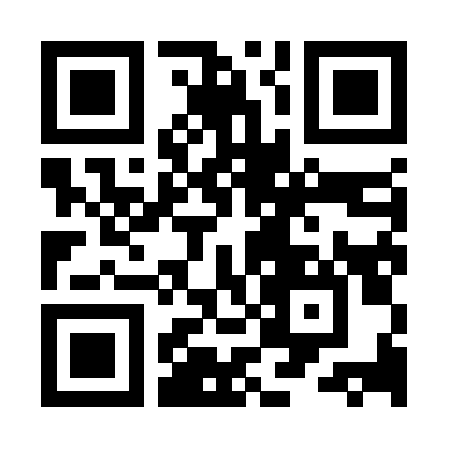
\includegraphics[scale=0.4]{pics/qr_Dupuit.eps} 
}

\begin{equation} \label{eq:dupui_1}
q=\frac{2\pi kh\left(P_e-P_w\right)}{\mu\left(\ln{\dfrac{r_e}{r_w}}\right)}
\end{equation}


В приведенном выражения использованы единицы СИ. 

Здесь 

$u_r$ - приведенная скорость фильтрации на расстоянии $r$ от скважины, м/с 

$q$ - объемные дебит скважины в рабочих условиях, м$^3$/с

$r$ -  радиус - расстояние от центра скважины, м

$r_e$ -  радиус зоны дренирования, на котором поддерживается постоянное давление, м

$r_w$ - радиус скважины, на котором замеряется забойное давление, м

$P$ - давление, Па

$P_e$ - давление на внешнем контуре дренирования, Па

$P_w$ - давление на забое скважины, Па

$k$ - проницаемость, м$^2$

$\mu$ - вязкость нефти в зоне дренирования, Па с

\

На практике часто бывает удобнее пользоваться значениями в практических метрических единицах измерения. 

\begin{equation} \label{eq:dupui_2}
q=\frac{kh\left(P_e-P_w\right)}{ 18.4 \mu\left(\ln{\dfrac{r_e}{r_w}}\right)}
\end{equation}

где 

$q$ - объемные дебит скважины в рабочих условиях, м$^3$/сут

$r$ -  радиус - расстояние от центра скважины, м

$r_e$ -  радиус зоны дренирования, на котором поддерживается постоянное давление, м

$r_w$ - радиус скважины, на котором измеряется забойное давление, м

$P$ - давление, атм

$P_e$ - давление на внешнем контуре дренирования, атм

$P_w$ - давление на забое скважины, атм

$k$ - проницаемость, мД

$\mu$ - вязкость нефти в зоне дренирования, сП

\

Далее если не указано особо будем использовать практические метрические единицы.


Выражение \ref{eq:dupui_2} можно переписать в виде

\begin{equation}
	P_{r} = P_{res} - 18.41\dfrac{ Q\mu B }{kh} \left[ \ln\dfrac{r_e}{r} +S \right]
\end{equation}

который удобен для расчёта распределения давления в пласте $P_r$ на произвольном расстоянии от скважины $r$.
В выражении (2) задано граничное значение давления $p_e$ на контуре $r_e$. Расчёт позволит найти любое значение внутри контура, в том числе и забойное давление $P_{wf}$ на $r=r_w$

Выражение можно переписать 
\begin{equation}
	P_{r} = P_{wf} + 18.41\dfrac{ Q\mu B }{kh} \left[ \ln\dfrac{r}{r_w} +S \right]
\end{equation}

где по известному дебиту и забойному давлению можно найти давление в пласте. При известном пластовом давлении можно оценить радиус контура на котором оно достигается.

\begin{figure}[h!]
	\begin{center}
		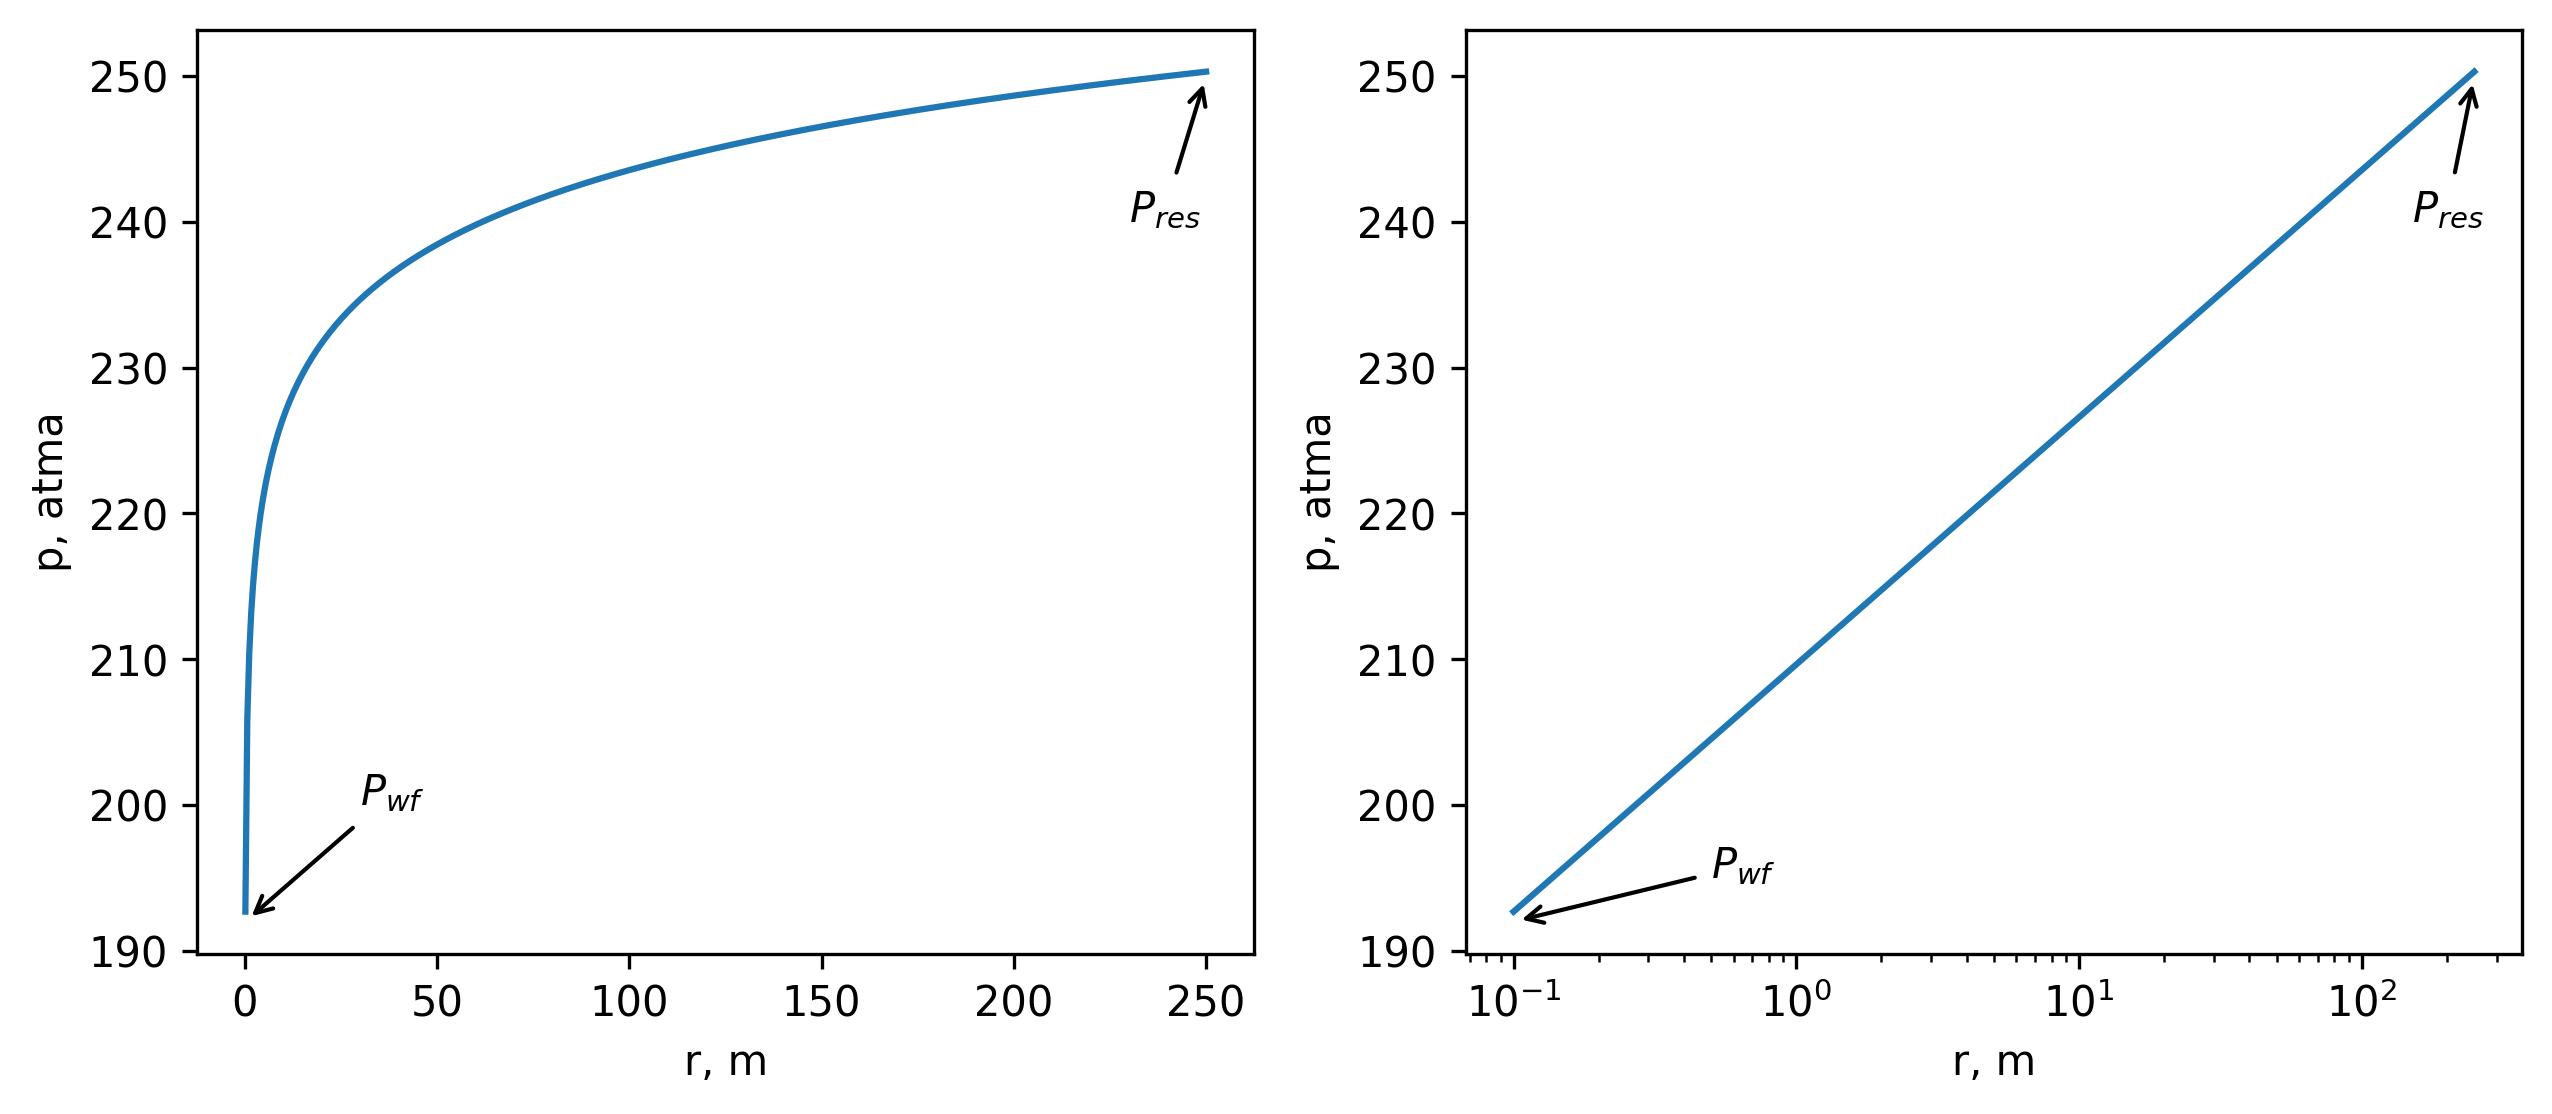
\includegraphics[width=12cm]{pics/stac_pressure_dist_1.png}
		\caption{Распределение давления в круговом пласте}
		\label{ris:stac_pressure_dist_1}
	\end{center}
\end{figure}


\subsection{Формула Дюпюи в декартовых координатах}
Для построения карты распределения давлений в пласте полезно вспомнить, что расстояние от скважины с координатами $(x_{well}, y_{well})$ до произвольной точки пласта с координатами $(x,y)$ можно найти по формуле 
$$r=\sqrt{ (x-x_{well})^2 + (y-y_{well})^2 }$$

Тогда выражение для расчета давления в любой точке пласта примет вид

\begin{equation} \label{eq:dupui_3}
	P_{r} = P_{res} - 18.41\dfrac{ Q\mu B }{kh} \left[ \ln\dfrac{r_e}{\sqrt{ (x-x_{well})^2 + (y-y_{well})^2 }} +S \right]
\end{equation}

Выражение \ref{eq:dupui_3} можно использовать, например, для построения карты распределения давления в пласте вокруг скважины. Можно применить следующий алгоритм для практической реализации - создать пустую матрицу со значениями давления по сетке координат вокруг скважины и перебирая все точки на сетке/матрице рассчитать карту давлений. Значения в сетке далее можно использовать для визуализации или последующих расчетов.


\section{Производительность скважины}

Уравнение производительности скважины можно записать в виде

\begin{equation} \label{eq:well_productivity}
	Q = T \Delta P J_D
\end{equation}

где
\begin{itemize}
	\item $Q$ - дебит жидкости скважины на поверхности, приведенный к стандартным условиям, м$^3$/сут. $$Q = qB$$
	
	\item $T$ - параметр зависящий от гидропроводности пласта 
	\begin{equation} \label{eq:T}
		T=\dfrac{18.41\mu B q }{\ k h}
	\end{equation}
	
	\item $\Delta P$ - депрессия на пласт, атм 
	\begin{equation} \label{eq:dP}
		\Delta P = \left(P_e-P_w\right)
	\end{equation}
	
	
	\item $J_D$ - безразмерный коэффициент продуктивности скважины, 
	\begin{equation} \label{eq:JD}
		J_D = \dfrac{1}{ \left(\ln{\dfrac{r_e}{r_w}} + S\right)}
	\end{equation}
	
	
\end{itemize}

Уравнение (\ref{eq:well_productivity}) можно интерпретировать следующим образом. Параметр $T$ отвечает за свойства пласта и флюида на которые трудно повлиять в ходе эксплуатации. Это то, что дала природа в точке где находится скважина. Депрессия $\Delta P$ -- параметр которым можно управлять в ходе эксплуатации регулируя забойное давление. Например за счет установки насоса и задания параметров его работы. На этом параметре должно быть сосредоточено основное внимание при анализе работы скважины. Параметр $J_D$ -- определяет качество соединения скважины с пластом или качество заканчивания. Его мы можем выбирать при строительстве скважины и можем менять в ходе эксплуатации проводя ГТМ, хотя и достаточно большой ценой. Поскольку мы можем влиять на $J_D$ важно понимать, какое оптимальное значение продуктивности можно достичь на конкретной скважине и как его можно изменить. 

Задачей гидродинамических исследований является установление величин $T$ и $J_D$, хотя традиционно речь ведется об определении проницаемости $k$ и скин-фактора $S$. 

\section{Учет скин-фактора}

Скин-фактор — гидродинамический параметр, характеризующий дополнительное фильтрационное сопротивление течению флюидов в околоскважинной зоне пласта, приводящее к изменению добычи (дебита) по сравнению с совершенной (идеальной) скважиной. Скин-фактор может приводить как к снижению дебита (например при загрязнении ПЗС), так и увеличению (образование высокопроводящих каналов в ПЗС).

Концепция скин-фактора получила широкое распространение на практике. Все инженеры-нефтяники знают этот параметр и оперируют им на практике. 

Изначально скин-фактор был введен как параметр учитывающий изменение проницаемости (загрязнение) призабойной зоны при расчете производительности скважины. Такое загрязнение может быть вызвано различными причинами:
\begin{itemize}
	\item проникновением бурового раствора в пласт и блокировкой поровых каналов;
	\item набуханием глин при контакте с фильтратом бурового раствора;
	\item химическим осаждением элементов бурового раствора, жидкости глушения или пластовых флюидов в призабойной зоне скважины, например осаждением солей или асфальтенов;
	\item продвижением песчаных частиц к стволу скважины;
	\item повреждением породы при перфорации;
	\item другими причинами.
\end{itemize}	

Для модели загрязненной призабойной зоны величину скин-фактора можно выразить формулой Хокинса \cite{Hawkins_1956}. Скин-фактор для плоскорадиального установившегося потока несжимаемой жидкости:

\begin{equation} \label{eq:skin_hokins}
S =\left( \frac{k}{k_s} -1\right)\ ln\frac{r_s}{r_w}
\end{equation}

здесь:

$k_s$ - проницаемость в загрязненной ПЗП;

$k$ - однородная проницаемость по всему пласту;

$r_s$ - радиус загрязненной зоны;

$r_w$ - радиус скважины.

\

\begin{figure}[h!]
	\begin{center}
		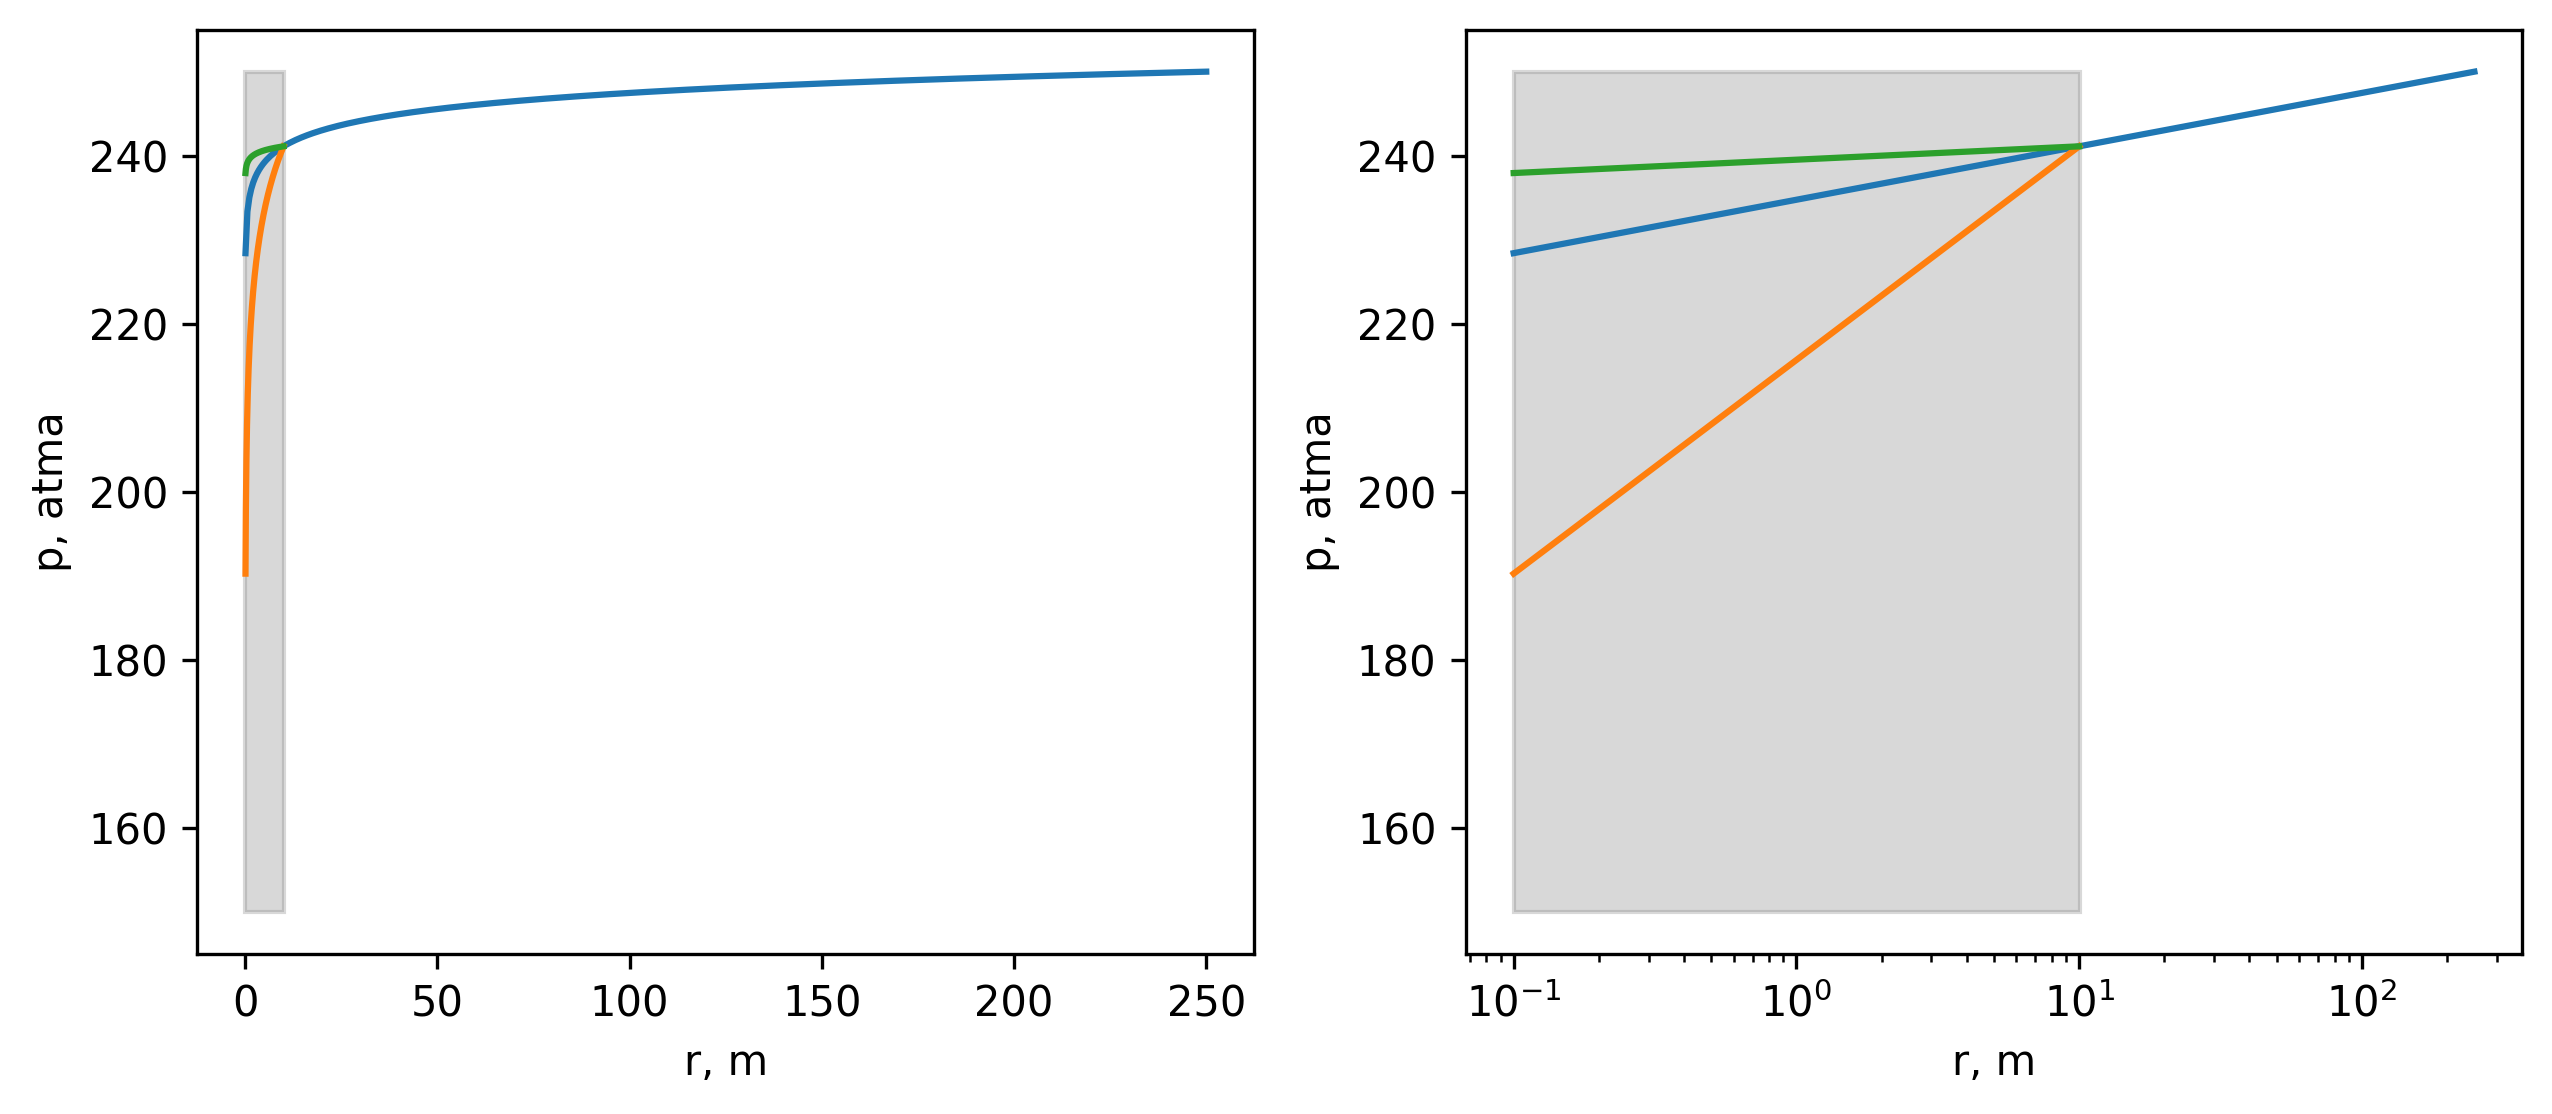
\includegraphics[width=12cm]{pics/stac_pressure_dist_skin.png}
		\caption{Изменение давления около скважины для загрязненной и простимулированной призабойной зоны}
		\label{ris:stac_pressure_dist_skin}
	\end{center}
\end{figure}

Концепция скин-фактора оказалась удобной для описания характеристики соединения скважины и пласта и была распространена на другие случаи, когда производительность скважины могла отличаться от производительности идеальной скважины:
\begin{itemize}
	\item для горизонтальных скважин;
	\item для скважин вскрывающих пласт под углом;
	\item для скважин пересеченных трещиной ГРП;
	\item для скважин вскрытых перфорацией и учета гидравлического сопротивления потока на перфорационных отверстиях;
	\item другими причинами.
\end{itemize}

Для многих подобных случаев предположение о радиальном притоке к скважине не верно, но величину скин-фактора используют, так как она позволяет сравнить производительность скважины со сложным заканчиванием с простой вертикальной скважиной. В таких случая говорят о псевдорадиальном скин-факторе - такой величине скин-фактора $S$, которая обеспечила бы такую же производительность для вертикальной скважины полностью вскрывающей пласт. 

Для стационарной радиальной модели притока учет скин-фактора приводит к следующим соотношениям:

\begin{equation} \label{eq:dupui_skin_1}
(P_e - P_{wf}) = \frac{18.4\mu q }{\ k h}(\ln\frac{r_e}{r_w}+S) 
\end{equation}


\begin{equation} \label{eq:dupui_skin_2}
q=\frac{kh\left(P_e-P_w\right)}{18.4 \mu\left(\ln{\dfrac{r_e}{r_w}} + S\right)}
\end{equation}

Скин-фактор может принимать как положительные, так и отрицательные значения. Причем если положительные значения не ограничены по величине и могут быть сколь угодно большими (по крайней мере с формальной точки зрения), то отрицательные значения не могут быть по модулю больше чем $\ln{\dfrac{r_e}{r_w}}$.

Расчет с отрицательными значениями скин-фактора не всегда оказывается удобен в практических реализациях. В таких случаях вместо скин-фактора можно использовать "эффективным радиусом" $r_{eff}$, что даст эквивалентное решение. 

\begin{equation}
	r_{eff} = r_w e^{-S}
\end{equation}

%Продуктивность скважины определяется как:
%$$J_{ss} = \frac{q_s}{P_e - P_{wf}} = \frac{k h}{18.41\mu B(\ ln\frac{r_e}{r_w} + S)} $$


%Скин фактор и нестационарное решение
%$$ P(r, t) = P{t} - \frac {9.205\mu {q_s} B }{k h}(\ ln\frac {k t}{ \phi \mu {c_t} {r^2}} +7.12 + 2S) $$

\section{Решение для постоянного давления на круговой границе с учетом среднего давления в области дренирования}

\begin{figure}[h!]
	\begin{center}
		

\tikzset{every picture/.style={line width=0.75pt}} %set default line width to 0.75pt        

\begin{tikzpicture}[x=0.75pt,y=0.75pt,yscale=-1,xscale=1]
%uncomment if require: \path (0,300); %set diagram left start at 0, and has height of 300

%Curve Lines [id:da7511541250087521] 
\draw [line width=1.5]    (344.45,238) .. controls (359.67,59.33) and (472.6,85.33) .. (563.2,79) ;
%Curve Lines [id:da025905206061745956] 
\draw [line width=1.5]    (321.55,238) .. controls (302.33,60.67) and (177,81.33) .. (102.8,79) ;
%Straight Lines [id:da6790536850628852] 
\draw  [dash pattern={on 0.84pt off 2.51pt}]  (321.55,60) -- (321.55,238) ;
%Straight Lines [id:da4154351528354687] 
\draw  [dash pattern={on 0.84pt off 2.51pt}]  (344.45,60) -- (344.45,238) ;
%Straight Lines [id:da012417840094577581] 
\draw  [dash pattern={on 4.5pt off 4.5pt}]  (102.8,92.67) -- (563.2,92.67) ;
%Straight Lines [id:da923812897272561] 
\draw    (102.8,42.67) -- (102.8,238) ;
%Straight Lines [id:da9720690336089455] 
\draw    (563.2,37) -- (563.2,238) ;

% Text Node
\draw (354.45,216.4) node [anchor=north west][inner sep=0.75pt]    {$r_{w}$};
% Text Node
\draw (545.2,216.4) node [anchor=north west][inner sep=0.75pt]    {$r_{e}$};
% Text Node
\draw (543.2,57.4) node [anchor=north west][inner sep=0.75pt]    {$p_{e}$};
% Text Node
\draw (547.2,97.07) node [anchor=north west][inner sep=0.75pt]    {$\overline{p}$};
% Text Node
\draw (380,131.4) node [anchor=north west][inner sep=0.75pt]    {$p( r)$};


\end{tikzpicture}
		\caption{Схема радиального притока к скважине при наличии постоянного давления на границе}
		\label{ris:radial_inflow_steady_state_average_pressure}
	\end{center}
\end{figure}

В приведенное выражение входит значение давления на контуре, которым не всегда бывает удобно пользоваться. В практических случаях значение на контуре трудно оценить, контур зоны дренирования может значительно отличаться от кругового, да и радиус оценить может быть сложно. Удобнее пользоваться средним давлением в зоне дренирования $\bar{P}$, которое может быть оценено по материальному балансу (смотри рисунок \ref{ris:radial_inflow_steady_state_average_pressure}). 



%[[вывод уравнения фильтрации для постоянного давления на границе с использованием среднего давления]]
В этом случае выражение для дебита примет вид
$$q=\frac{kh\left( \bar{P}-P_w\right)}{ 18.41 \mu\left(\ln{\dfrac{r_e}{r_w}}  - \dfrac{1}{2}+ S \right)}$$


\section{Решение для круговой непроницаемой границы}

Схема модели радиального притока для условия непротекания на круговой границе приведена на рисунке \ref{ris:radial_inflow_steady_state_2}.

\begin{figure}[h!]
	\begin{center}
		

\tikzset{every picture/.style={line width=0.75pt}} %set default line width to 0.75pt        

\begin{tikzpicture}[x=0.75pt,y=0.75pt,yscale=-1,xscale=1]
%uncomment if require: \path (0,542); %set diagram left start at 0, and has height of 542

%Shape: Rectangle [id:dp9986954540947564] 
\draw  [color={rgb, 255:red, 74; green, 144; blue, 226 }  ,draw opacity=1 ] (275.5,106.5) -- (410.5,106.5) -- (410.5,167.5) -- (275.5,167.5) -- cycle ;
%Shape: Circle [id:dp6552629065863149] 
\draw  [color={rgb, 255:red, 74; green, 144; blue, 226 }  ,draw opacity=1 ][fill={rgb, 255:red, 255; green, 255; blue, 255 }  ,fill opacity=1 ] (275.5,361.5) .. controls (275.5,324.22) and (305.72,294) .. (343,294) .. controls (380.28,294) and (410.5,324.22) .. (410.5,361.5) .. controls (410.5,398.78) and (380.28,429) .. (343,429) .. controls (305.72,429) and (275.5,398.78) .. (275.5,361.5) -- cycle ;
%Shape: Circle [id:dp8082105624253089] 
\draw   (225.5,361.5) .. controls (225.5,296.61) and (278.11,244) .. (343,244) .. controls (407.89,244) and (460.5,296.61) .. (460.5,361.5) .. controls (460.5,426.39) and (407.89,479) .. (343,479) .. controls (278.11,479) and (225.5,426.39) .. (225.5,361.5) -- cycle ;
%Shape: Rectangle [id:dp8805209935477971] 
\draw   (225.5,106.5) -- (460.5,106.5) -- (460.5,167.5) -- (225.5,167.5) -- cycle ;
%Shape: Rectangle [id:dp9848620821804102] 
\draw  [color={rgb, 255:red, 255; green, 255; blue, 255 }  ,draw opacity=1 ][fill={rgb, 255:red, 255; green, 255; blue, 255 }  ,fill opacity=1 ] (328,96) -- (358,96) -- (358,117) -- (328,117) -- cycle ;
%Shape: Circle [id:dp7806087558343378] 
\draw   (328,361.5) .. controls (328,353.22) and (334.72,346.5) .. (343,346.5) .. controls (351.28,346.5) and (358,353.22) .. (358,361.5) .. controls (358,369.78) and (351.28,376.5) .. (343,376.5) .. controls (334.72,376.5) and (328,369.78) .. (328,361.5) -- cycle ;
%Straight Lines [id:da7744729507427655] 
\draw  [dash pattern={on 0.84pt off 2.51pt}]  (225.5,167.5) -- (225.5,361.5) ;
%Straight Lines [id:da34517185100966685] 
\draw  [dash pattern={on 0.84pt off 2.51pt}]  (460.5,167.5) -- (460.5,361.5) ;
%Straight Lines [id:da3585865226685445] 
\draw    (328,86.5) -- (328,106.5) ;
%Straight Lines [id:da41145580018262384] 
\draw    (358,86.5) -- (358,106.5) ;
%Straight Lines [id:da4626155220696013] 
\draw  [dash pattern={on 0.84pt off 2.51pt}]  (343,106.5) -- (343,361.5) ;
%Straight Lines [id:da5723626081572117] 
\draw    (343,361.5) -- (408.75,452.82) ;
\draw [shift={(410.5,455.25)}, rotate = 234.25] [fill={rgb, 255:red, 0; green, 0; blue, 0 }  ][line width=0.08]  [draw opacity=0] (7.14,-3.43) -- (0,0) -- (7.14,3.43) -- cycle    ;
%Straight Lines [id:da9257805385062015] 
\draw    (343,361.5) -- (401.22,385.36) ;
\draw [shift={(404,386.5)}, rotate = 202.29] [fill={rgb, 255:red, 0; green, 0; blue, 0 }  ][line width=0.08]  [draw opacity=0] (7.14,-3.43) -- (0,0) -- (7.14,3.43) -- cycle    ;
%Straight Lines [id:da15606395599455936] 
\draw    (346,186.5) -- (407.5,186.5) ;
\draw [shift={(410.5,186.5)}, rotate = 180] [fill={rgb, 255:red, 0; green, 0; blue, 0 }  ][line width=0.08]  [draw opacity=0] (7.14,-3.43) -- (0,0) -- (7.14,3.43) -- cycle    ;
\draw [shift={(343,186.5)}, rotate = 0] [fill={rgb, 255:red, 0; green, 0; blue, 0 }  ][line width=0.08]  [draw opacity=0] (7.14,-3.43) -- (0,0) -- (7.14,3.43) -- cycle    ;
%Straight Lines [id:da6156171963471699] 
\draw    (346,208.5) -- (457.5,208.5) ;
\draw [shift={(460.5,208.5)}, rotate = 180] [fill={rgb, 255:red, 0; green, 0; blue, 0 }  ][line width=0.08]  [draw opacity=0] (7.14,-3.43) -- (0,0) -- (7.14,3.43) -- cycle    ;
\draw [shift={(343,208.5)}, rotate = 0] [fill={rgb, 255:red, 0; green, 0; blue, 0 }  ][line width=0.08]  [draw opacity=0] (7.14,-3.43) -- (0,0) -- (7.14,3.43) -- cycle    ;
%Straight Lines [id:da29225849394418124] 
\draw    (343,86.5) -- (343,60.75) ;
\draw [shift={(343,57.75)}, rotate = 450] [fill={rgb, 255:red, 0; green, 0; blue, 0 }  ][line width=0.08]  [draw opacity=0] (7.14,-3.43) -- (0,0) -- (7.14,3.43) -- cycle    ;
%Straight Lines [id:da05244651066444139] 
\draw    (264.9,137) -- (283.1,137) ;
\draw [shift={(286.1,137)}, rotate = 180] [fill={rgb, 255:red, 0; green, 0; blue, 0 }  ][line width=0.08]  [draw opacity=0] (7.14,-3.43) -- (0,0) -- (7.14,3.43) -- cycle    ;
%Straight Lines [id:da42364169594920353] 
\draw    (423.95,137) -- (400.1,137) ;
\draw [shift={(397.1,137)}, rotate = 360] [fill={rgb, 255:red, 0; green, 0; blue, 0 }  ][line width=0.08]  [draw opacity=0] (7.14,-3.43) -- (0,0) -- (7.14,3.43) -- cycle    ;
%Straight Lines [id:da523288490832504] 
\draw    (516,109.5) -- (516,164.5) ;
\draw [shift={(516,167.5)}, rotate = 270] [fill={rgb, 255:red, 0; green, 0; blue, 0 }  ][line width=0.08]  [draw opacity=0] (7.14,-3.43) -- (0,0) -- (7.14,3.43) -- cycle    ;
\draw [shift={(516,106.5)}, rotate = 90] [fill={rgb, 255:red, 0; green, 0; blue, 0 }  ][line width=0.08]  [draw opacity=0] (7.14,-3.43) -- (0,0) -- (7.14,3.43) -- cycle    ;

% Text Node
\draw (336.5,38.9) node [anchor=north west][inner sep=0.75pt]    {$q$};
% Text Node
\draw (361,84.9) node [anchor=north west][inner sep=0.75pt]    {$r_{w}$};
% Text Node
\draw (254,117.4) node [anchor=north west][inner sep=0.75pt]    {$q$};
% Text Node
\draw (423.5,117.4) node [anchor=north west][inner sep=0.75pt]    {$q$};
% Text Node
\draw (369,166.9) node [anchor=north west][inner sep=0.75pt]    {$r$};
% Text Node
\draw (428,186.9) node [anchor=north west][inner sep=0.75pt]    {$r_{e}$};
% Text Node
\draw (318.5,327.4) node [anchor=north west][inner sep=0.75pt]    {$r_{w}$};
% Text Node
\draw (391.5,365.9) node [anchor=north west][inner sep=0.75pt]    {$r$};
% Text Node
\draw (403,425.4) node [anchor=north west][inner sep=0.75pt]    {$r_{e}$};
% Text Node
\draw (463.5,182.4) node [anchor=north west][inner sep=0.75pt]    {$p_{e}$};
% Text Node
\draw (527,129.4) node [anchor=north west][inner sep=0.75pt]    {$h$};


\end{tikzpicture}
		\caption{Схема радиального притока к скважине при наличии непроницаемой границы}
		\label{ris:radial_inflow_steady_state_2}
	\end{center}
\end{figure}

При условии непротекания давления на границе условия стационарности (неизменности давления) не достигаются. При работе скважины с постоянным дебитом забойное давление будет постоянно снижаться. Однако начиная с некоторого момента, когда влияние скважины достигнет границ - давление в всей области дренирования начнет снижаться равномерно (смотри рисунок \ref{ris:radial_pss_dynamics}). 

\begin{figure}[h!]
	\begin{center}
		

\tikzset{every picture/.style={line width=0.75pt}} %set default line width to 0.75pt        

\begin{tikzpicture}[x=0.75pt,y=0.75pt,yscale=-1,xscale=1]
%uncomment if require: \path (0,300); %set diagram left start at 0, and has height of 300

%Shape: Axis 2D [id:dp9842834583970732] 
\draw  (121,262.2) -- (555.3,262.2)(140.76,53) -- (140.76,278.2) (548.3,257.2) -- (555.3,262.2) -- (548.3,267.2) (135.76,60) -- (140.76,53) -- (145.76,60)  ;
%Curve Lines [id:da6767694694353563] 
\draw    (143,80) .. controls (229.3,79.2) and (347.3,106.2) .. (491.3,133.2) ;
%Curve Lines [id:da1513616030724707] 
\draw [color={rgb, 255:red, 208; green, 2; blue, 27 }  ,draw opacity=1 ]   (143,80) .. controls (188.3,142.2) and (269.7,145.25) .. (487.7,185.25) ;
%Straight Lines [id:da13598982031442275] 
\draw    (289,98) -- (289,145.25) ;
\draw [shift={(289,148.25)}, rotate = 270] [fill={rgb, 255:red, 0; green, 0; blue, 0 }  ][line width=0.08]  [draw opacity=0] (7.14,-3.43) -- (0,0) -- (7.14,3.43) -- cycle    ;
\draw [shift={(289,95)}, rotate = 90] [fill={rgb, 255:red, 0; green, 0; blue, 0 }  ][line width=0.08]  [draw opacity=0] (7.14,-3.43) -- (0,0) -- (7.14,3.43) -- cycle    ;
%Straight Lines [id:da13673864754675735] 
\draw    (409.5,121) -- (409.5,168.25) ;
\draw [shift={(409.5,171.25)}, rotate = 270] [fill={rgb, 255:red, 0; green, 0; blue, 0 }  ][line width=0.08]  [draw opacity=0] (7.14,-3.43) -- (0,0) -- (7.14,3.43) -- cycle    ;
\draw [shift={(409.5,118)}, rotate = 90] [fill={rgb, 255:red, 0; green, 0; blue, 0 }  ][line width=0.08]  [draw opacity=0] (7.14,-3.43) -- (0,0) -- (7.14,3.43) -- cycle    ;

% Text Node
\draw (264,114.4) node [anchor=north west][inner sep=0.75pt]    {$\Delta p$};
% Text Node
\draw (384.5,135.9) node [anchor=north west][inner sep=0.75pt]    {$\Delta p$};
% Text Node
\draw (471,107.9) node [anchor=north west][inner sep=0.75pt]    {$p_{e}$};
% Text Node
\draw (471,185.9) node [anchor=north west][inner sep=0.75pt]    {$p_{wf}$};
% Text Node
\draw (528,239.4) node [anchor=north west][inner sep=0.75pt]    {$t$};


\end{tikzpicture}
		\caption{Изменение давления на границе и на забое скважины во времени}
		\label{ris:radial_pss_dynamics}
	\end{center}
\end{figure}

Такой режим, при котором забойное давление меняется, но перепад давления $P_e - P_w$ остается постоянным называют псевдо-установившимся режимом работы (pss - pseudo steady state). 

Для псевдо-установившегося режима можно записать выражение

$$q=\frac{kh\left(P_e-P_w\right)}{ 18.41 \mu\left(\ln{\dfrac{r_e}{r_w}} - \dfrac{1}{2} + S\right)}$$
где 

$q$ - объемные дебит скважины в рабочих условиях, м3/сут;

$r$ -  радиус - расстояние от центра скважины, м;

$r_e$ -  радиус зоны дренирования, на котором поддерживается постоянное давление, м;

$r_w$ - радиус скважины, на котором замеряется забойное давление, м;

$P$ - давление, атм;

$P_e$ - давление на внешнем контуре дренирования, атм;

$P_w$ - давление на забое скважины, атм;

$k$ - проницаемость, мД;

$\mu$ - вязкость нефти в зоне дренирования, сП.

\

\subsection{Решение для круговой непроницаемой границы с учетом среднего давления в зоне дренирования}

Аналогично случаю для постоянного давления на границе можно переписать выражение с использованием среднего давления в области дренирования. 

$$q=\frac{kh\left( \bar{P}-P_w\right)}{ 18.41 \mu\left(\ln{\dfrac{r_e}{r_w}} - \dfrac{3}{4}+ S \right)}$$

%[[Вывод уравнений для псевдо-установившегося режима работы]]



\section{Стационарные решения для вертикальной скважины в резервуаре произвольной формы}

Здесь уравнения и методы расчета для горизонтальных, наклонно направленных скважин, скважин с ГРП, горизонтальных скважин с МГРП. 

\begin{equation}
	q=\frac{kh\left( \bar{P}-P_w\right)}{ 18.41 \mu\left(\ln{\dfrac{2.2458 A}{C_A r_w^2}} + S \right)}
\end{equation}

$q$ - объемные дебит скважины в рабочих условиях, м3/сут;

$A$ -  площадь области дренирования, м$^2$;

$C_A$ -  фактор формы, зависит от формы резервуара и расположения скважины;

$r_w$ - радиус скважины, на котором замеряется забойное давление, м;

$\bar{P}$ - среднее давление в области дренирования, атм;

$P_e$ - давление на внешнем контуре дренирования, атм;

$P_w$ - давление на забое скважины, атм;

$k$ - проницаемость, мД;

$\mu$ - вязкость нефти в зоне дренирования, сП.

\

\begin{figure}[h!]
	\centering
	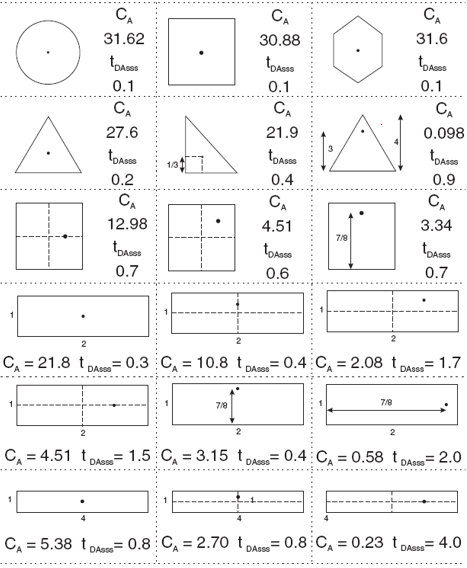
\includegraphics[width= 10cm]{pics/shape_factors.png} 
	\label{fig:shape_factors}
	\caption{Значения фактора формы}
\end{figure}

%todo -надо переделать рисунок и добавить ссылки на источники

Безразмерное время достижения псевдо-установившегося режима притока, определяемое видом резервуара

$$t_{DApss} = \frac{kt_{pss}}{\varphi \mu c_t A} $$

\section{Стационарные решения для скважины с трещиной ГРП}

%todo надо расписать четче и привести решение и для трещины конечной проводимости
Для больших времен скважину с трещиной ГРП можно представить как скважину с увеличенным "эффективным радиусом" $r_{eff}$, или, что эквивалентно, как скважину с отрицательным скин-фактором.

\begin{equation}
	r_{eff} = r_w e^{-S}
\end{equation}

Это верно, только если $x_f << r_e$

Для трещины бесконечной проводимости 

\begin{equation}
	r_{eff} = \frac{x_f}{2}
\end{equation}

тогда 

\begin{equation}
	S = \frac{2r_w}{x_f}
\end{equation}




\section{Суперпозиция для стационарного решения}

\subsection{Суперпозиция для нескольких скважин с постоянным дебитом} 

Для стационарного решения работает принцип суперпозиции - сумма двух решений также будет решением, это позволяет построить карту для нескольких скважин.
Давление в любой точке пласта можно найти по формуле

\begin{equation}
	P_{res} - P_{x,y} =  \sum_{i} 18.41\dfrac{ Q_i\mu B }{kh} \left[ \ln\frac{r_e}{\sqrt{ (x-x_{w.i})^2 + (y-y_{w.i})^2 }} +S \right]
\end{equation}

Выражение справедливо только если $\sqrt{ (x-x_{w.i})^2 + (y-y_{w.i})^2 }< r_e$.

\subsection{Суперпозиция для нескольких скважин с постоянным забойным давлением}

При наличии нескольких скважин можно записать выражение для оценки забойных давлений скважин


$$
P_{res} - P_{wf.j} =  \sum_{i} 18.41\dfrac{ Q_i\mu B }{kh} \left[ \ln\dfrac{r_e}{\sqrt{ (x_{w.j}-x_{w.i})^2 + (y_{w.j}-y_{w.i})^2 }} +S \right]
$$

Если считать забойные давления $P_{wf.j}$ известными а дебиты скважин $Q_i$ не известными, тогда выражение (6) можно рассматривать как систему линейных алгебраических уравнений вида

$$AX = B$$

Где
$$
A_{[i,j]} = 18.41\dfrac{ \mu B }{kh} \left[ \ln\dfrac{r_e}{\sqrt{ (x_{w.j}-x_{w.i})^2 + (y_{w.j}-y_{w.i})^2 }} +S \right]
$$

$$
B_{[j]}=P_{res} - P_{wf.j}
$$

такую систему можно решить например с использованием пакета `scipy.linalg` 

\section{Задания для самостоятельной работы}

Для совершенствования навыков работы с python выполните следующие задания:

1. Постройте график распределения давления в пласте для композитного пласта. В композитном пласте на расстоянии $r<r_1$ проницаемость равна $k=k_1$, а для $r>=r_1$, $k=k_2$. 

2. Постройте двумерную тепловую или контурную карту распределения давления в пласте для моделей однородного и композитного пласта.

3. Рассчитайте среднюю величину давления в круговой области дренирования для однородного пласта. Насколько среднее давление в круговой области дренирования будет отличаться от давления на контуре. Чему будет равен коэффициент $S$ в выражении  $Q=\dfrac{kh}{18.41\mu B} \dfrac{P_{res}-P_{wf}}{ln(\dfrac{r_e}{r_w})+S}$ при использовании вместо давления на контуре среднего давления? Постройте график, на котором будет отображаться распределение давления в зоне дренирования и величина среднего давления (в виде линии).

4. Для примера с несколькими скважинами имитирующими трещину ГРП рассчитайте дебиты скважин таким образом, чтобы забойное давление на всех скважинах было одинаковым. Постройте графики распределения давления в пласте. Постройте график дебитов вдоль "скважины".


	
	
	
	\chapter{Простые нестационарные решения уравнения фильтрации}
	
	Для установившегося режима фильтрации давление в пласте не меняется. Для псевдо-установившегося режима постоянным остается перепад давления между пластом и забоем. После запуска, остановки или изменения режима работы скважины эти условия не выполняются. Давление в различных точках пласта может меняться по разному. Такой режим называют неустановившимся, а решения его описывающие нестационарными (зависят от времени).

Неустановившиеся решения уравнения фильтрации (transient solutions) представляют значительный практический интерес во многих задачах, включая задачи интерпретации ГДИС. В тоже время они относительно сложны и требуют применения компьютерных алгоритмов. В данном пособие проведение расчетов иллюстрируется с использованием макросов для Excel -- Unifloc VBA.

\section{Решение линейного стока}

Для решения уравнения фильтрации - линейного дифференциального уравнения в частных производных второго порядка необходимо задать начальные и граничные условия. 

Самое простое решение можно получить для случая вертикальной скважины бесконечно малого радиуса запускающейся с постоянным дебитом. Условия соответствующие этому случаю можно выразить следующим образом:

\begin{itemize}
	\item Начальное условие. До запуска скважины в момент времени  $t_D = 0$ давление в пласте равно начальному во всех точках $p=p_i$
	$$ t_D < 0, p_D = 0 $$ 
	\item Граничное условие на скважине.  Условие постоянства дебита на скважине можно трансформировать в граничное условие опираясь на закон Дарси.
	$$ \lim_{r_D \to 0} {r_D \frac{\partial p_D}{\partial r_D}} = -1$$
	\item Граничное условие на бесконечном расстоянии от скважины. Давление в пласте на бесконечно большом расстоянии от скважины равно начальному.
	$$ r_D = \infty, p_D = 0$$
\end{itemize}

\begin{figure}[h!]
	\begin{center}
		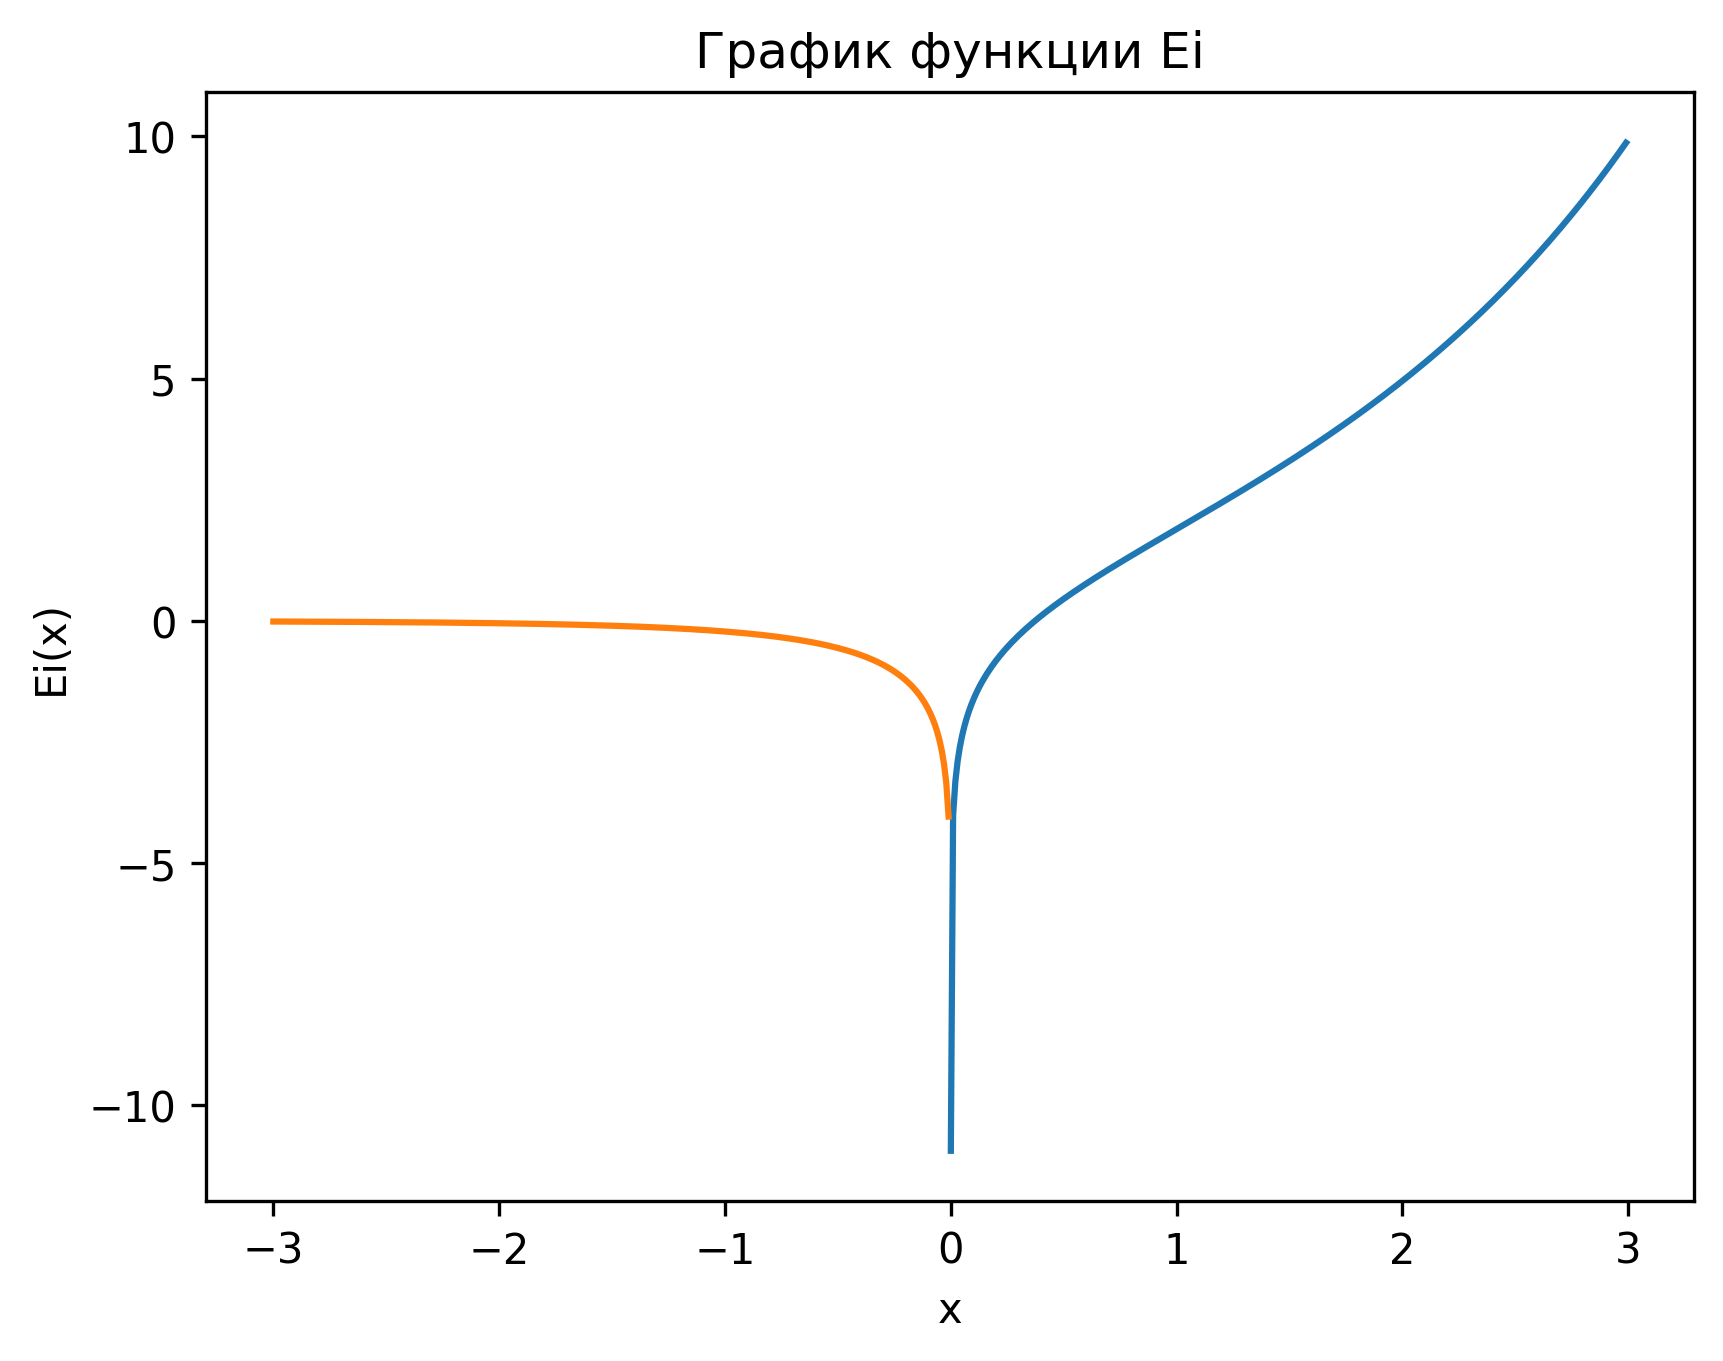
\includegraphics[width=12cm]{pics/Ei_plot_1.png}
		\caption{График функции Ei}
		\label{ris:Ei_plot_1}
	\end{center}
\end{figure}

\begin{figure}
	%\begin{figure}[h!]
	\begin{center}
		\begin{tikzpicture}
			\begin{axis}
				[axis lines = left,
				 width = 0.98\textwidth,
				%xlabel=$x$,
				%ylabel={$Ei_1(x)$},
				]
				\addplot gnuplot[no markers, samples=100, domain = 0:10]{expint(1,x)};
				\addlegendentry{$Ei_1(x)$}
			\end{axis}
		\end{tikzpicture}
		\caption{График функции интегральной экспоненты $Ei_1(x)$.}
		\label{ris:ei1}
	\end{center}
	%\end{figure}
\end{figure}



В этом случае решение может быть выражено через функцию интегральной экспоненты 
\begin{equation}
	p_D(r_D,t_D) = - \frac{1}{2} Ei \left(- \dfrac{ r_D^2}{4t_d} \right)
\end{equation} 

где $-Ei(-x)$ - интегральная показательная функция, рисунок \ref{ris:Ei_plot_1}.

$$Ei(x)=-\int\limits_{x}^{\infty}\frac{e^{-t}}{t}\,\mathrm dt$$

\marginpar{
	\href{https://www.wolframalpha.com/input/?i=Ei\%28x\%29}{$Ei(x)$ Wolfram Alpha} 
	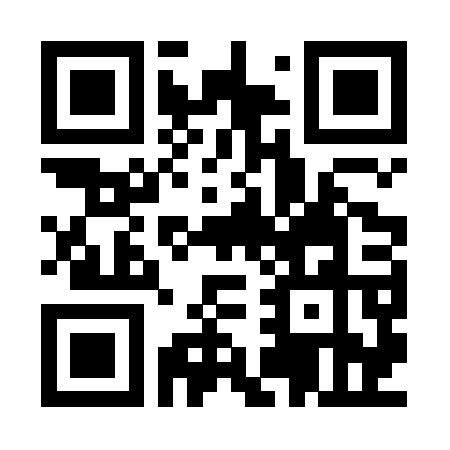
\includegraphics[scale=0.4]{pics/qr_ei_wolfram.eps} 
	}

Часто для проведения расчетов, особенно с использованием компьютерных библиотеке расчетов, бывает удобнее пользоваться модифицированной интегральной показательной функцией $Ei_1(x)$ или $E_1(x)$ или $Ei_n(x)$ при $n=1$.
 $$Ei_n(x) = \int\limits_{1}^{\infty}\frac{e^{-tx}}{t^n}\,\mathrm dt $$

График интегральной показательной функции $Ei_1(x)$ приведен на рисунке \ref{ris:ei1}.
Для вещественных положительных $x\in\mathbb R, x>0$ верно $E_1(x) = - Ei( -x)$

Функцию интегральной экспоненты можно представить в виде ряда. 

$$Ei(x)=-\int\limits_{x}^{\infty}\frac{e^{-t}}{t}\,\mathrm dt=\gamma+\operatorname{ln}|-x|+\sum\limits_{n\ge1}\frac{{-x}^n}{n!\cdot n}, \;  x\in\mathbb R,\;$$

\begin{figure}
	%\begin{figure}[h!]
	\begin{center}
		\begin{tikzpicture}
			\begin{axis}
				[axis lines = left,
				width = 0.98\textwidth,
				%xlabel=$x$,
				%ylabel={$f(x)$},
				]
				\addplot gnuplot[no markers, samples=100, domain = 0:2]{expint(1,x)};
				\addlegendentry{$Ei_1(x)$}
				\addplot gnuplot[no markers, samples=100, domain = 0:2]{-log(x)-0.5772};
				\addlegendentry{$ln(x)$}
			\end{axis}
		\end{tikzpicture}
		\caption{Сравнение функций интегральной экспоненты $E_1(x)$ и $ln(x)$.}
		\label{ris:ei2}
	\end{center}
	%\end{figure}
\end{figure}

Из приведенного выражения можно сделать выводы, что для маленьких значений аргумента  функция интегральной экспоненты $E_1(x)$ может быть аппроксимирована логарифмической зависимостью. 

$$E_1(x) = -ln(x) - \gamma $$

График сравнения функций $E_1(x)$ и $ln(x)$ показан на рисунке \ref{ris:ei2}. Видно, что хорошей аппроксимация будет только для маленьких значений аргумента $x < 0.01$. Но для решения уравнения фильтрации именно эта зона представляет наибольший интерес.

%\begin{wrapfigure}{r}{0.5\textwidth}
\begin{figure}[h!]
	\begin{center}
		\begin{tikzpicture}
			\begin{axis}
				[axis lines = left,
				width = 0.98\textwidth,
				xlabel=$x$,
				ylabel={$f(x)$},
				xmode=log,
				log ticks with fixed point,
				]
				\addplot gnuplot[no markers, samples=100, domain = 0.00001:20 ]{expint(1,x)};
				\addlegendentry{$Ei_1(x)$}
				\addplot gnuplot[no markers, samples=100, domain = 0.00001:20]{-log(x)-0.5772};
				\addlegendentry{$ln(x)$}
			\end{axis}
		\end{tikzpicture}
		\caption{Сравнение функций интегральной экспоненты $E_1(x)$ и $ln(x)$ в логарифмическом масштабе.Можно оценить диапазон применимости логарифмической аппроксимации.}
		\label{ris:ei3}
	\end{center}
\end{figure}
%\end{wrapfigure}

Представление интегральной экспоненты в виде логарифмической аппроксимации удобно на практике, так как логарифм легче вычислять. В большинстве языков программирования и инструментов для проведения расчетов расчет логарифма реализован по умолчанию. А для расчета интегральной экспоненты, часто приходится предпринимать дополнительные шаги.

Решение уравнения фильтрации для линейного стока с учетом логарифмической аппроксимации можно представить в виде 

\begin{equation}
p_D(r_D,t_D) = \frac{1}{2} \left( ln \left( \dfrac{ t_D }{r_D^2}  \right) +0.809 \right) 
\end{equation}


при использовании данного уравнения, следует помнить, что приближенное решение применимо при $\dfrac{r_D^2}{4t_D} < 0.01$

Решение линейного стока в размерных переменных

\begin{equation}
p\left(r,t\right)=p_i-\frac{18.41q_sB\mu}{kh}\left(-\frac{1}{2}Ei\left(-\frac{\varphi\mu c_tr^2}{0.00144kt}\right)\right) 
\end{equation}

Решение с учетом логарифмической аппроксимации в размерных переменных

\begin{equation}
p\left(r,t\right)=p_i-\frac{9.205q_sB\mu}{kh}\left(ln{\frac{kt}{\varphi\mu c_tr^2}}-7.12\right)
\end{equation}

верно при 
$$\frac{kt}{\varphi\mu c_tr^2}>70000 $$

Решения приведены для практических метрических единиц измерения, что можно увидеть по размерному коэффициенту. 

Нестационарное решение с учетом скин-фактора будет иметь вид


\begin{equation} 
P(r, t) = P_{i} - \frac {9.205 {q_s} B\mu }{k h}(\ ln\frac {k t}{ \varphi \mu {c_t} {r^2}} -7.12 + 2S) 
\end{equation}


%\subsubsection{Радиус исследования}
%Надо бы тут описать концепцию радиуса исследований и подходы к его оценке

\subsubsection{Расчет в Unifloc VBA}

Следующие функции реализованы в Unifloc VBA

\begin{verbatim}
	Ei
	E_1
\end{verbatim}	

Описания функций и из аргументов можно найти в руководстве пользователя  Unifloc VBA



\section{Радиус влияния скважины}


Нестационарное решение в безразмерных переменных
$$ 
p_D(r_D,t_D) = - \frac{1}{2} Ei \left(- \dfrac{ r_D^2}{4t_d} \right)
$$
где безразмерные переменные введены как
$$ r_D = \frac{r}{r_w}  $$
$$ t_D = \frac{0.00036 kt}{\phi \mu c_t r_w^2}  $$
$$ p_D = \frac{kh}{ 18.41 q_s B \mu} \left( p_i - p \right)   $$

Здесь использование единицы измерения СИ.
- $r_w$ - радиус скважины, м

- $r$ - расстояние от центра скважины до точки в пласте, м

- $q_s$ - дебит скважины на поверхности, приведенный к нормальным условиям м3/сут

- $\phi$ - пористость, доли единиц

- $\mu$ - вязкость нефти в пласте, сП

- $B$ - объемный коэффициент нефти, м3/м3

- $p_i$ - начальное давление в пласте, атм

- $p$ - давление на расстоянии $r$, атм

- $c_t$ - общая сжимаемость системы в пласте, 1/атм

Для этих же безразмерных переменных, считая начальное давление равным давлению на контуре можно записать стационарное решение для движения в круговом пласте

$$p_D = \ln r_{eD} - \ln r_D $$

сравним это решение с логарифмической аппроксимацией (1)

$$p_D(r_D,t_D) = - \frac{q_D}{2} \left[ \ln \left( \dfrac{ r_D^2}{4t_d} \right) +\gamma \right] $$

которое можно преобразовать к виду
$$p_D(r_D,t_D) = - q_D \ln r_D  + \frac{q_D}{2} \left[ \ln(4t_D)   -\gamma \right] $$

сравнивая со стационарным решением можно найти выражение безразмерного радиуса контура в зависимости от безразмерного времени
$$\ln r_{eD} = \frac{1}{2}(\ln(4t_D)-\gamma) $$

$$r_{eD} =  \sqrt { 4t_D e^{-\gamma} }  $$

наконец получим
$$r_{eD} = \sqrt {2.2458 t_D} $$

это значение называют радиусом влияния скважины. Используя это значение для определенного момента времени можно получить стационарное распределение давления в системе хорошо приближающее решение линейного стока работающего в бесконечном пласте. Можно считать это расстояние на которое распространяется влияние скважины.

достижение радиуса влияния внешних границ будет обуславливать начало перехода от неустановившегося режима фильтрации к режиму обусловленному влиянием границ - стационарному для границы постоянного давления или псевдо установившемуся для непроницаемой границы.

\begin{figure}[h!]
	\begin{center}
		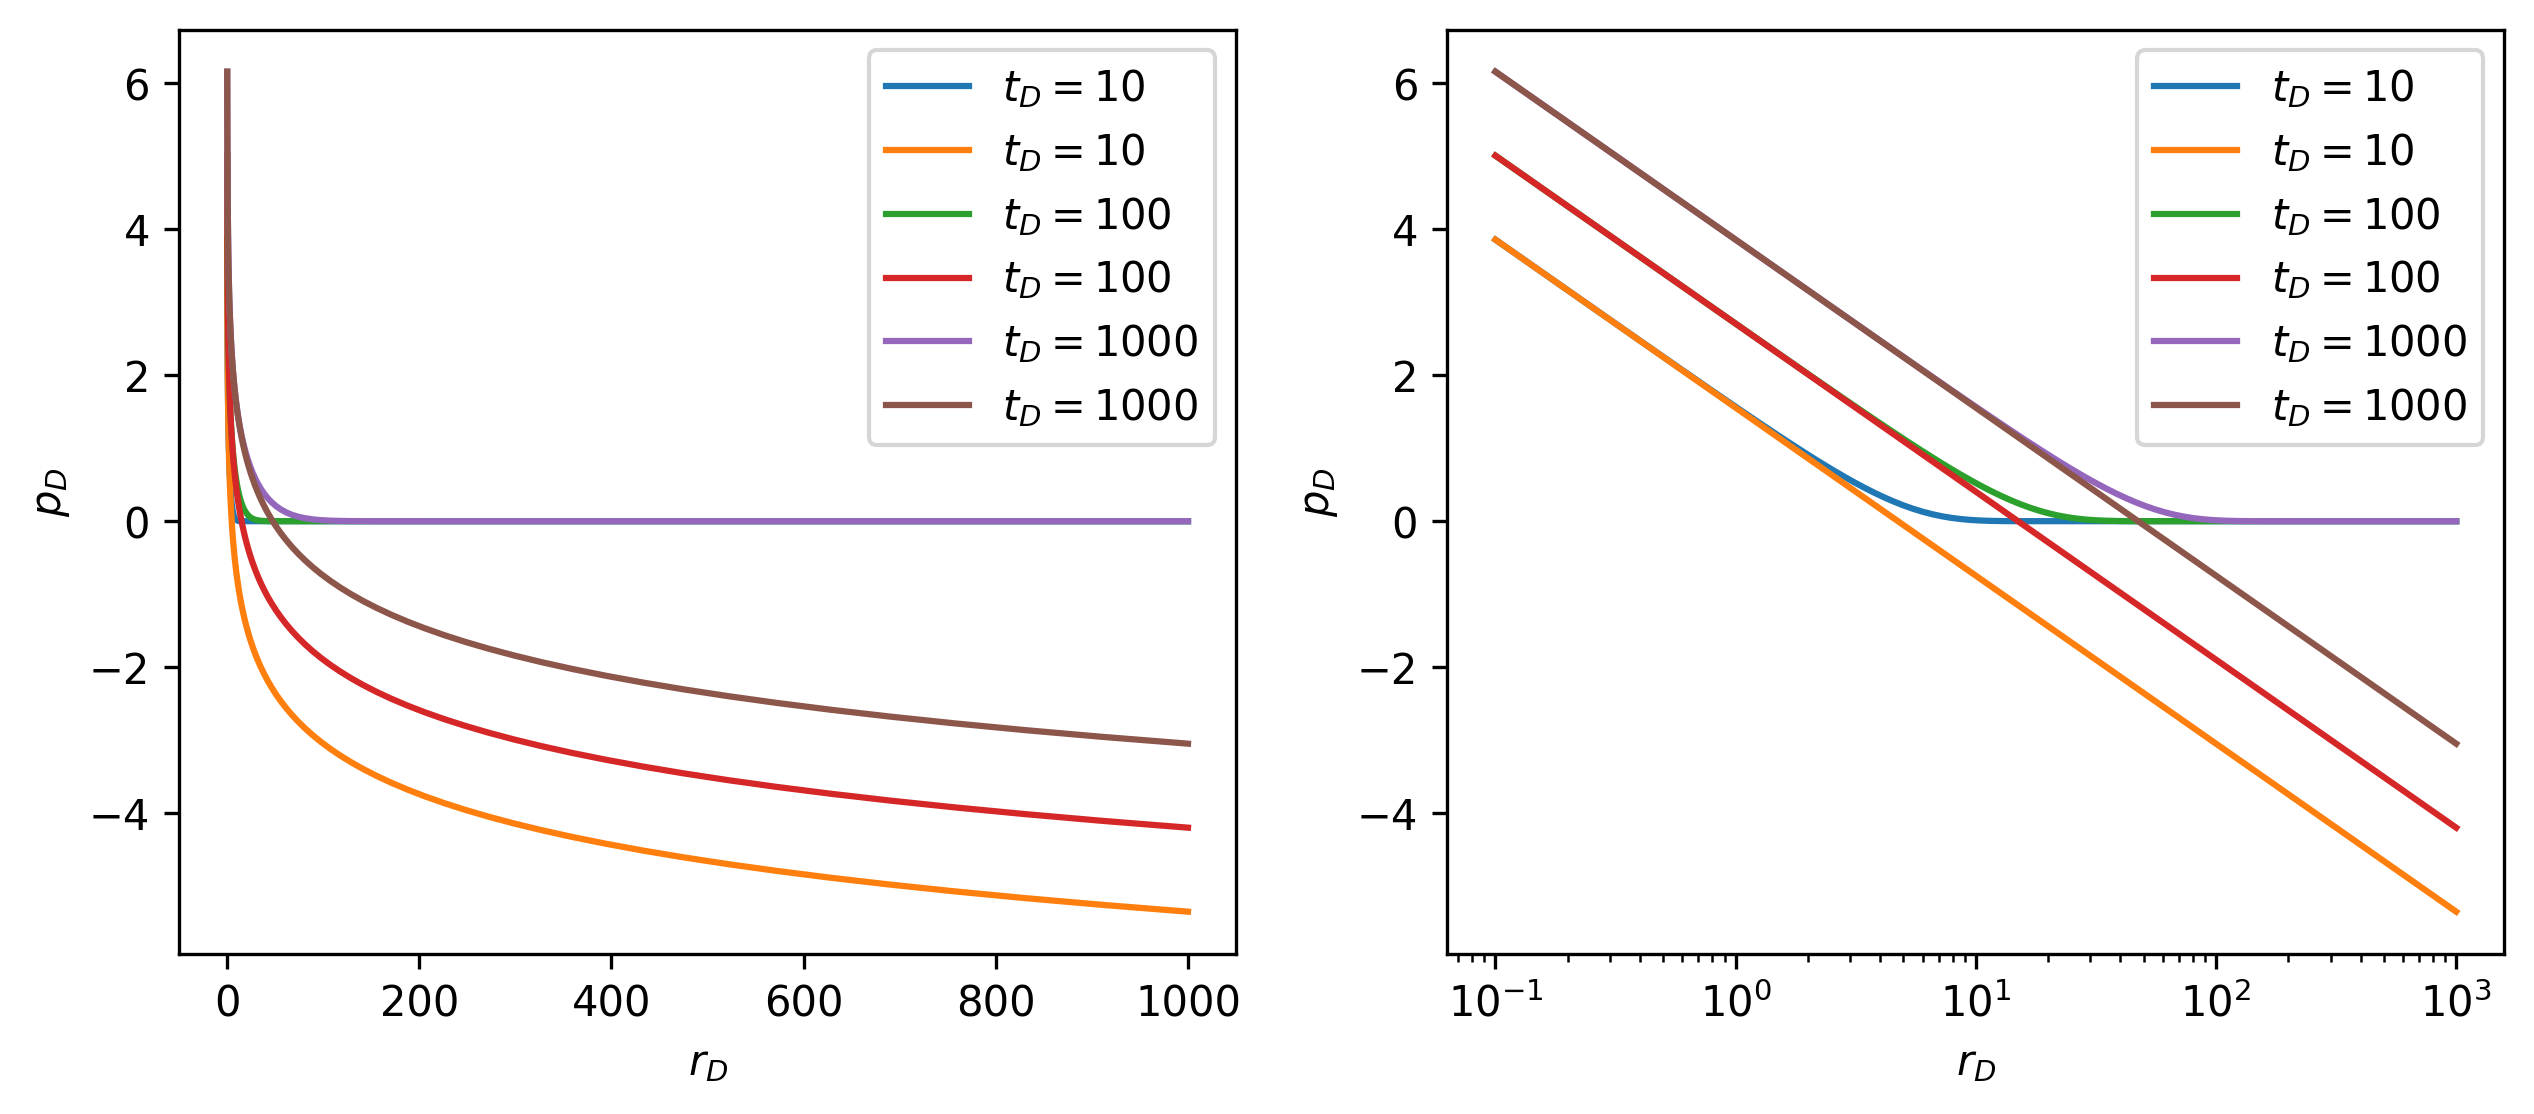
\includegraphics[width=12cm]{pics/stac_radius_investigation_1.png}
		\caption{Изменение радиуса влияния скважины со временем. Сравнение стационарного и нестационарного решений}
		\label{ris:stac_radius_investigation_1}
	\end{center}
\end{figure}



\section{Решение для конечного радиуса скважины}
Для получения сложных решений уравнения фильтрации часто используется преобразование Лапласа.
\marginpar{
	\href{https://qrgo.page.link/ZUfT2}{преобразование Лапласа} 
	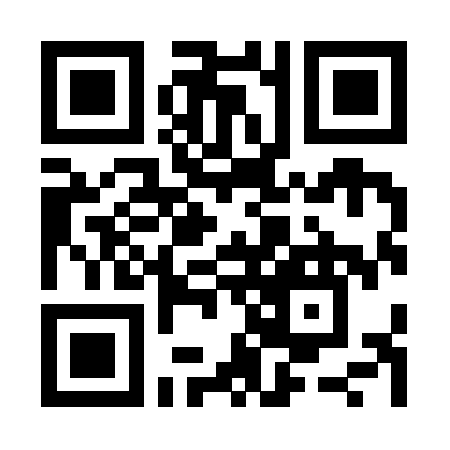
\includegraphics[scale=0.4]{pics/qr_Laplace.eps} 
}

$$ L \left [ f(t) \right] = \tilde{f}(s) = \int_{0}^{\infty}f(t)e^{-st}dt $$

где $s$ параметр пространства Лапласа соответствующий времени

Решение для бесконечно малого радиуса скважины в пространстве Лапласа будет иметь вид

\begin{equation}  \label{eq:laplace_solution_1}
\tilde{p}_D(s) = \frac{1}{s} K_0 \left( r_D \sqrt s  \right) 
\end{equation}

решение для конечного радиуса скважины \cite{Everdingen_1949}

\begin{equation} \label{eq:laplace_solution_2}
	\tilde{p}_D(s) = \frac{K_0 \left( r_D \sqrt{s}  \right) }{ s \sqrt{s} K_1 \left( \sqrt s  \right)  }
\end{equation}

где 

$K_0$, $K_1$ - модифицированные функции Бесселя;

\marginpar{
	\href{https://qrgo.page.link/hkh7x}{модифицированные функции Бесселя} 
	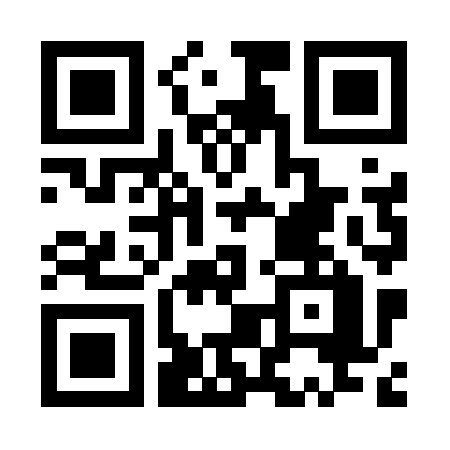
\includegraphics[scale=0.4]{pics/qr_Bessel.eps} 
}

$s$ - переменная пространства Лапласа;

$\tilde{p}_D(s)$ - изображение функции ${p}_D$ в пространстве Лапласа;

$r_D$ - безразмерный радиус скважины.

\

Перевод решения из пространства Лапласа в обычное пространство не всегда возможен аналитически. В современных условиях перевод делается численно с использованием компьютеров, что позволяет строить и исследования решения уравнения фильтрации при различных условиях. 

Широко распространено применения алгоритма Стефеста для численного обратного преобразования Лапласа. 

\subsubsection{Расчет в Unifloc VBA}

Следующие функции реализованы в Unifloc VBA

\begin{verbatim}
	transient_pd_radial
	transient_pwf_radial_atma
\end{verbatim}	

Описания функций и из аргументов можно найти в руководстве пользователя  Unifloc VBA

\section{Учет влияния ствола скважины}
Часто управление дебитом скважины производится на поверхности -- за счет регулировки на скважинной арматуре. При этом, например, перекрытие потока на скважинной арматуре не сразу приведет к прекращению притока из пласта на забое скважины. Для скважины оснащенной насосом со свободным динамическим уровнем приток из пласта будет продолжаться пока не заполнится затрубное пространство скважины. Для фонтанирующей скважины с пакером тот же эффект, хотя и заметно менее выраженный будет наблюдаться из за высокой сжимаемость газожидкостной смеси в стволе скважины. 

Эффект различия скоростей изменения дебита жидкости на устье и забое называют эффектом влияния ствола скважины или эффектом послепритока (wellbore storage). Он часто встречается, оказывает большое влияние на качество исследования и обязательно должен учитываться при интерпретации и моделировании исследований.

Простейший вариант учета эффекта послепритока описывается с использованием постоянного коэффициента послепритока или коэффициента влияния ствола скважины $C_s$, определяющего "сжимаемость" жидкости в стволе скважины.

$$ C_s = - \frac{ \Delta V}{ \Delta p} $$

Для фонтанирующей скважины:

Изменение объема жидкости в стволе скважины происходит за счет сжимаемости жидкости:

$$ \Delta V = -c{V_w}{\Delta P} $$

$$ C_s = - \frac{ \Delta V}{ \Delta p} $$

Для фонтанирующей скважины, коэффициент ствола скважины:

$$ C_s =  c {V_w} $$

$ V_w $ - объем жидкости в стволе скважины  [м$^3$]
$c$ - сжимаемость жидкости или газожидкостной смеси в стволе скважины [1/атм]

%todo нужен пример расчета с числами для скважины с разными значениями давления - где газа много и мало, где пакер есть и пакера нет

Влияние ствола в механизированной скважине:

$$ C_s = - \frac{ \Delta V}{ \Delta p} $$
$$ {\Delta V} = A_{cas}{\Delta h} $$
$$ {\Delta P} ={ro g}{\Delta h}$$
$$ C_s =  \frac{ A_{cas}}{ \Delta p} $$

$ A_{cas}$ - площадь поперечного сечения затрубного пространства, [м$^2$]


$ {\Delta h}$ - изменение уровня жидкости в затрубном пространстве, [ м ]

Решение уравнения фильтрации с учетом скин-фактор и послепритока
Для решения линейного стока граничное условие соответствующее послепритоку с постоянным $C_s$ можно записать как

$$ \lim_{r_D \to 0} {r_D \frac{\partial p_D}{\partial r_D}} = -1 + \left. C_D \frac{\partial p_D}{\partial t_D} \right|_{t_D=1}$$

Предположим, что у нас имеется решение задачи запуска скважины с постоянным дебитом в прострастве Лапласа без учета скин-фактора и послепритока $\tilde{p}_D^{*}$. Где $s$ параметр пространства Лапласа соответствующий $t_D$.

Например для бесконечного пласта и скважины нулевого радиуса такое решение имеет вид: 

$$\tilde{p}_D^*(s) = \frac{1}{s} K_0 \left( r_D \sqrt s  \right) $$

Тогда решение с учетом скин-фактора и послепритока может быть выражено 

$$\tilde{p}_D(s) = \frac{s \tilde{p}_D^* + S}{s \left( 1+s C_D \left( s \tilde{p}_D^* + S \right)  \right)}   $$



%\subsubsection{Решение для постоянного забойного давления}
%
%\subsubsection{Решение для скважины с ГРП}
%
%Надо привести решение для скважины с ГРП
%
%\subsubsection{Решение для скважины с горизонтальной скважиной}
%
%Надо привести решение для горизонтальной скважины


\section{Суперпозиция для нестационарных решений}


Большинство моделей используемых при интерпретации ГДИС основаны на линеаризованном дифференциальном уравнении в частных производных - уравнении фильтрации (уравнении пьезопроводности или диффузии).

$$ \frac{\partial ^2 p }{\partial r^2} + \frac{1}{r} \frac{\partial p}{\partial r} = \frac{\varphi \mu c_t}{k} \frac{\partial p}{\partial t} $$

Для линейных уравнений справедлив принцип суперпозиции - линейная комбинация решений также является решением. То есть если $f(t,r)$ и $g(t,r)$ являются решениями, то $\alpha f(t,r) + \beta g(t,r)$  также является решением.

Это позволяет строить сложные решения уравнения фильтрации на основе простых.

\subsection{Расчет кривой восстановления давления}

Один из самых простых примеров применения суперпозиции. Предполагаем, что добывающая скважина в однородном изотропном пласте запускается в момент времени $t=0$ и работает $t_{p}$ часов, после чего останавливается. После остановки скважины забойное давление растет - и мы получим кривую восстановления давления.

Пусть решение задачи запуска скважины (падения давления) будет $P_D(t_D, r_D)$. Тогда решение для изменения давления при запуске и последующей остановки скважины можно представить в виде 

\begin{equation}
	P_{bu.D}(t_D, t_{prod.D}, r_D) = P_D(t_D) - P_D(t_D-t_{prod.D}, r_D) \cdot \mathcal{H}(t_D-t_{prod.D}) 
\end{equation}

где

- $t_D$ - безразмерное время после запуска скважины,

- $t_{prod.D}$ - безразмерное время работы скважины после запуска

- $\mathcal{H}$ - ступенчатая функция Хевисайда \url{https://ru.wikipedia.org/wiki/Функция_Хевисайда} (в некоторых книгах обозначается как $\theta$)

- $P_D(t_D, r_D)$ - безразмерное давление - решение задачи запуска скважины (падения давления)

- $P_{bu.D}(t_D, t_{prod.D}, r_D)$ - безразмерное давление- решение задачи запуска  и последующей остановки скважины

Для проведения векторных расчетов в python удобно выражение с использованием функции Хевисайда

$$ \mathcal{H} = \begin{cases}0 & x < 0\\1 & x = 0\\1 & x > 0\end{cases}$$

Применение функции Хевисайда позволяет избежать в расчетных функциях условных операторов в явном виде для отдельных элементов входных массивов. Это потенциально ускоряет расчет. 



\subsubsection{Решение для остановки скважины (КВД)}

Для наших целей определим принцип суперпозиции следующим образом: перепад давления в любых точках пласта определяется как сумма перепадов давлений в этих точках, вызванных работой отдельных скважин на залежи. 

Пусть известно решение уравнения фильтрации для запуска скважины с постоянным дебитом в невозмущенном пласте   $p(t)$. 

Известно, что скважина запустилась с дебитом $q$ на период времени $t_p$ и потом остановилась. Требуется найти зависимость изменения давления в скважине после остановки.

$$ p_{D}^{bu}(\Delta t)=p_D(t_p +\Delta t) - p_D(\Delta t)$$  при $\Delta t > 0$

Пример 1.

Рассмотрим случай, когда добывающая скважина работает в различные периоды времени при некоторых постоянных дебитах, как показано на рисунке.  



Итак, рассматривается скважина, работающая с постоянным дебитом $q_1$ в интервале времени от 0 до $t_1$, затем в момент времени $t_1$ дебит изменился и стал равным $q_2$, а при времени $t_2$ дебит вновь изменился и стал равным $q_3$.

Наша задача состоит в определении функции давления на стенке скважины в период времени $t>t_2$.

Для решения этой задачи так же, как и ранее, применим метод суперпозиции, но не в виде учета интерференции соседних скважин, а в виде суммирования дополнительных перепадов давления в самой рассматриваемой скважине:

То есть рассматривается работа нескольких скважин, находящихся в одной точке, но запущенных в работу в разное время. Решение получено для начального дебита $q_1$, за полученное время $t_n$. В момент времени $t_1$ запускается в работу новая скважина с точным известным месторасположением и начальным дебитом $ \left(q_2 - q_1\right)$,так , что чистый дебит скважины после времени  $t_1$ будет равен  $q_2$.В момент времени $t_2$ запускается в работу новая скважина с точным известным месторасположением и начальным дебитом $ \left(q_3 - q_2\right)$, который превращается в дебит $q_3$ после времени $t_2$ …и т. д.

Общее снижение давления в скважине определится с учетом двух изменений дебита притока как:

\begin{eqnarray}
	\left( P_{пл} - P_c\right) = \left( \Delta P\right)_1 + \left( \Delta P\right)_2 +\left( \Delta P\right)_3 = \nonumber  \\ 
	= - \frac{q_1 \mu}{4\pi kh} \left( ln \frac{1,78 \mu m c_t r_c^2}{kt}-2S \right) - \nonumber  \\ 
	\frac{ \left(q_2 - q_1\right)\mu}{4\pi kh} \left( ln \frac{1,78 \mu m c_t r_c^2}{k\left(t-t_1\right)}-2S \right)- \nonumber  \\ 
	\frac{ \left(q_3 - q_2\right)\mu}{4\pi kh} \left( ln \frac{1,78 \mu m c_t r_c^2}{k\left(t-t_2\right)}-2S \right)
\end{eqnarray}

\subsection{Решение для произвольной истории дебитов (ступенчатое изменение дебита)} 

Для расчета изменения давления при переменном дебите введем произвольное референсное значение дебита $ q_{ref} $ (например первое не нулевое значение дебита при запуске скважины). Используем это значение для определения безразмерного давления.
$$ p_D = \frac{kh}{ 18.41 q_{ref} B \mu} \left( p_i - p \right) $$

и безразмерного дебита 

$$q_D = \frac{q}{q_{ref}} $$

Тогда, используя принцип суперпозиции, можем выписать выражение для изменения давления на скважине и вокруг нее для произвольного момента времени

\begin{equation}
	P_{mr.D}(t_D, r_D) = \sum_i \left[ q_{D(i)}-q_{D(i-1)} \right] \cdot p_D\left(t_D-t_{D(i)}, r_D\right)\cdot \mathcal{H}(t_D-t_{D(i)}) \tag{7} 
\end{equation}

где

- $i$ - индекс значения дебита в таблице изменения дебитов

- $q_{D(i)}$ - безразмерный дебит с номером $i$, который стартует в момент времени $t_i$. Для первого момента времени $i$ дебит следующий перед ним считается равным нулю

- $t_{D(i)}$ - безразмерный момент времени - включения дебита с номером $i$

- $t_{D}$ - безразмерный момент времени для которого проводится расчет

- $\mathcal{H}$ - ступенчатая функция Хевисайда

- $p_D\left(t\right)$ - зависимость безразмерного давление от времени - решение задачи запуска скважины с постоянным единичным дебитом

- $P_{mr.D} $ - безразмерное давление $P_{mr.D}(t_D, r_D)$ учитывающее историю изменения дебитов скважины

\subsection{Случай для произвольной истории дебитов (линейное изменение дебита)}

для линейно меняющегося дебита $dq_D t_D$ решение можно представить как интеграл

$$
p_D = \int_0^{t_D}{- \frac{dq_D}{2} Ei \left(- \dfrac{ r_D^2}{4t_d} \right) dt_D}
$$



Для линейно меняющегося дебита во времени (как и для любой другой зависимости) надо решение проинтегрировать по времени (надо бы подробнее расписать - сделать это позже, например как у Щелкачева в основах нестационарной фильтрации на стр 321).

Для линейной зависимости дебита от времени 
$$
Q_D = dQ_D \cdot t_D 
$$
можно получить выражение
$$
p_D(r_D,t_D, dQ_D) =-\frac{dQ_D t_D }{2} \left[ \left( 1+ \frac{r_D^2}{4 t_D} \right) Ei \left(- \dfrac{r_D^2}{4t_D} \right) + e^{-\dfrac{r_D^2}{4t_D}} \right] $$ 

где $dQ_D$ - скорость изменения дебита.

Для таблично заданных дебитов и времен можно оценить 

$$
dQ_{D(i)} = \dfrac{Q_{D(i)}-Q_{D(i-1)}}{t_{D(i)} - t_{D(i-1)} } 
$$

Cравните формулу (11) с формулой (9.68) в книге Щелкачева "Основы неустановившейся фильтрации"

Тогда, используя принцип суперпозиции, можем выписать выражение для изменения давления на скважине и вокруг нее для произвольного момента времени

$$P_{mr.D}(t_D, r_D) = \sum_i  p_D\left(t_D-t_{D(i)}, r_D, dQ_{D(i+1)} - dQ_{D(i)}\right)\cdot \mathcal{H}(t_D-t_{D(i)}) $$

где

- $i$ - индекс значения дебита в таблице изменения дебитов

- $dQ_{D(i)}$ - изменение безразмерного дебита относительно безразмерного времени (14.4) 

- $t_{D(i)}$ - безразмерный момент времени - включения дебита с номером $i$

- $t_{D}$ - безразмерный момент времени для которого проводится расчет

- $\mathcal{H}$ - ступенчатая функция Хевисайда

- $p_D\left(t\right)$ - зависимость безразмерного давление от времени - решение задачи запуска скважины с постоянным единичным дебитом

- $P_{mr.D} $ - безразмерное давление $P_{mr.D}(t_D, r_D)$ учитывающее историю изменения дебитов скважины

следует обратить внимание, при суперпозиции скорость изменения дебита вычисляется как $dQ_{D(i+1)} - dQ_{D(i)}$.  при реализации расчета необходимо предусмотреть, чтобы для первого и последнего шага расчет прошел корректно. Для этого можно, например, добавить к массивам дебитов и времени дополнительный значения в начале и в конце массивов соответствующие постоянным значениям дебита. 

Также надо учитывать, что в приведенном выражении массивы должны начинаться со значений $Q_D=0$





\subsection{Решение для скважины в пласте с непроницаемой границей}
надо добавить мнимую скважину

Пусть скважина, представленная на рисунке, находится на расстоянии L от прямолинейной непроницаемой границы, через которую отсутствует поток жидкости.



Математическая задача о работе скважины, находящейся на каком-то расстоянии L от непроницаемой прямолинейной границы, может быть рассмотрена как  работа двух скважин - данной и воображаемой, в данной случае добывающей, находящейся на расстоянии 2L от рассматриваемой. Воображаемая скважина работает с той же производительностью, что и фактическая скважина. Рассмотрение работы двухскважинной системы как аналога работы одной скважины с границей в пласте базируется на том, что равновесие двух рядом находящихся одинаково работающих скважин может наступить только при условии, что через линию, проходящую между скважинами и равноотстоящую от них, нет потока (то есть, градиент давление вдоль этой линии равен нулю). Таким образом можно записать работу двух скважин в бесконечном пласте в виде:

$$ P_{пл} - P_c = - \frac{q_A \mu}{4\pi kh} \left( ln \frac{1,67 \mu m c_t r_c^2}{kt}-2S \right)- \frac{q_B \mu}{4\pi kh} Ei \left( \frac{1,78 \mu c_t m \left(2L\right)^2}{4kt} \right)$$

Здесь также можно отметить, что в воображаемой скважине не принят во внимание скин - фактор, так как рассматривается влияние этой скважины на работу фактической скважины, находящийся на большем расстоянии от нее. 



Решение для скважины в пласте с границей постоянного давления 
Тут тоже надо добавить мнимую скважину и описать пример построения решения


\subsection{Другие применения принципа суперпозиции}
также можно добавить ряд других примеров

%скважине в секторе с двумя границами
%скважине в замкнутой области с несколькими границами 
%скважина с ГРП - метод источников
%группа скважин взаимодействующих между собой
%горизонтальная скважина
%горизонтальная скважина с ГРП

	
	
	
	
	
	%\insertbibliofull
	\printbibliography
	
	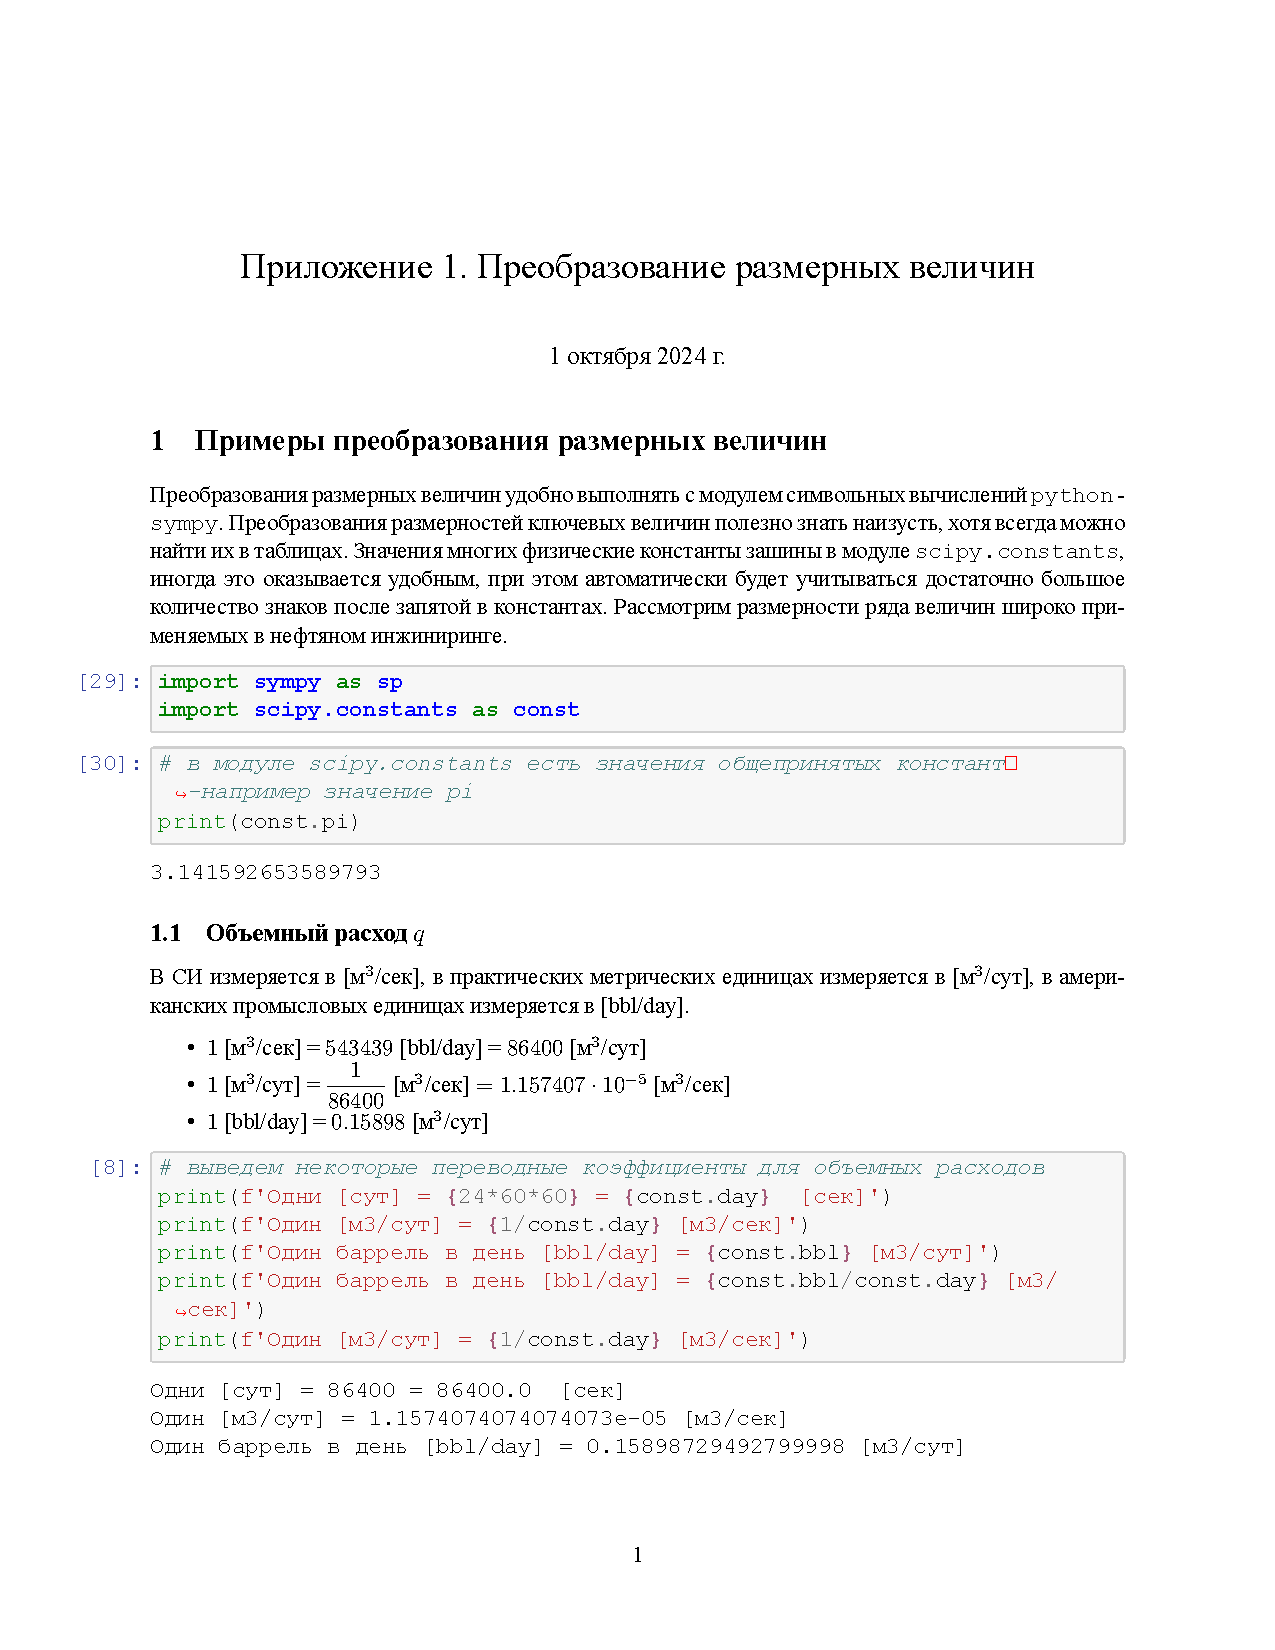
\includepdf[pages=-]{appendix/Приложение 1. Преобразование размерных величин.pdf}
	
\end{document}